\documentclass[11pt]{article}
\usepackage[margin=1in]{geometry}
\usepackage{amsmath,amssymb,amsthm,booktabs,mathtools}
\usepackage{graphicx}
\usepackage[hidelinks]{hyperref}
\pdfstringdefDisableCommands{\def\HH{H2}\def\st#1{}}
\usepackage{xcolor}
\newtheorem{theorem}{Theorem}[section]
\newtheorem{lemma}[theorem]{Lemma}
\newtheorem{proposition}[theorem]{Proposition}
\newtheorem{corollary}[theorem]{Corollary}
\theoremstyle{definition}
\newtheorem{definition}[theorem]{Definition}
\theoremstyle{remark}
\newtheorem{remark}[theorem]{Remark}
\newcommand{\HH}{\mathbb H^2}
\newcommand{\D}{\mathbb D}
\newcommand{\st}[1]{\textbf{[#1]}}
\usepackage{url}
\makeatletter\g@addto@macro{\UrlBreaks}{\do\.\do\_\do\-}\makeatother
\newcommand{\lean}[1]{\nolinkurl{#1}}
\newcommand{\Lan}{\mathcal L}
\setlength{\emergencystretch}{3em}
\allowdisplaybreaks

\title{Vortex rings and rows on the hyperbolic plane:\\ one stability boundary through the horocycle}
\author{Gordon Speagle\\\small Independent researcher, Boise, Idaho, USA}
\date{October 2026}

\begin{document}
\maketitle

\begin{abstract}
We study the linear stability of equally spaced point vortices of equal strength on the hyperbolic plane $\HH$, with the
true Green function $-\log\tanh(d/2)$ and no background vorticity (Kimura's model). For the regular $N$-ring the Hessian of
the augmented Hamiltonian splits into $2\times2$ Fourier blocks whose entries are rational in $\xi=\tanh^2(r/2)$, $r$ the
hyperbolic radius. From them we prove: rings with $N\le7$ are stable at every radius; every $N\ge8$ has exactly one threshold
radius, below which the ring is unstable in the mode $\lfloor N/2\rfloor$ and above which it is spectrally stable; and the
threshold is an algebraic number, certified to 45 digits for $8\le N\le16$. For odd $N\ge9$ there is a short window
(width $\sim10^{-8}$--$10^{-7}$ in $\xi$ for $N\le15$, $O(N^{-3})$ in general) where the ring is spectrally stable but
the Hessian is indefinite: the critical mode carries two eigenvalues of opposite Krein signature, so a definiteness
(energy--momentum) criterion misses stability there. For large $N$, $\cosh r_*(N)=N/\tau_\infty+O(1/N)$ and the arc spacing
at threshold tends to $\ell_*=2\pi/\tau_\infty=0.843908\ldots$, which is exactly the critical spacing of an infinite row on a
horocycle: that row is stable iff $\ell\ge\ell_*$, with no Krein window. Rows along hypercycles of geodesic curvature
$\kappa$ are unstable at every spacing iff $|\kappa|\le1/\sqrt2$; above it they are stable beyond one threshold
$\ell_{\rm hyp}(\kappa)$ (an interval-arithmetic certificate shows the threshold is unique), real-analytic on $(1/\sqrt2,1)$,
which blows up at $1/\sqrt2$ and ends at the horocycle point $(1,\ell_*)$, where the ring thresholds also accumulate. The boundary does not continue analytically through that point:
the hypercycle branch has a square-root branch point there and the even and odd ring thresholds arrive with different
finite slopes. Most statements are checked in Lean~4 with Mathlib; the rest are labelled as certified (interval or exact
arithmetic), derived or numerical.
\end{abstract}

\tableofcontents

%======================================================================
\section{Introduction}\label{sec:intro}

\paragraph{The problem.} A point vortex on a surface moves in the velocity field of the others; the motion is Hamiltonian,
with the Green function of the Laplacian as pair interaction and the area form as symplectic form. In the plane, the regular
ring of $N$ equal vortices (Thomson's polygon) is linearly stable for $N\le6$, neutral for $N=7$ and unstable for $N\ge8$
\cite{Havelock1931}, and the infinite straight row (a single von K\'arm\'an row) is unstable at every spacing
\cite{vonKarman1912,Lamb1932,Aref1995}. On a curved surface the ring has an extra parameter, its radius measured against the
curvature, and the question becomes: \emph{for which radii is the ring stable?} On the hyperbolic plane the question extends
naturally to rows: equally spaced vortices along any curve of constant geodesic curvature $\kappa$ (a geodesic, a
hypercycle, a horocycle or a circle) form a relative equilibrium, translating along the curve.

\paragraph{The model.} We use the Green function of the Laplace--Beltrami operator of $\HH$ (curvature $-1$) that vanishes at
infinity,
\[
G(d)=-\frac1{2\pi}\log\tanh\frac d2,
\]
$d$ the geodesic distance. Since $\HH$ is non-compact and homogeneous no compensating background vorticity is needed, the
Robin function is constant, and the Hamiltonian is the plain pair sum $H=-\sum_{j<k}\log\tanh(d_{jk}/2)$ (unit circulations,
factor $2\pi$ absorbed). This is the model attributed to Kimura~\cite{Kimura1999}; it is the case $\lambda=-1$ of the image
Green function of Montaldi--Tokieda~\cite[\S4.2]{MontaldiTokieda2013}, and Boatto~\cite{Boatto2008} uses the same Green function.
It differs from the ``sinh model'' $-\log\sinh(d/2)$ studied by Montaldi and Tokieda~\cite{MontaldiTokieda2013}, which
carries a uniform background vorticity (\S\ref{sec:prior}). The tanh interaction is screened beyond one curvature radius,
$-\log\tanh(d/2)\approx2e^{-d}$, and this changes the large-$N$ behaviour completely.

\paragraph{Results.} Write $\xi=\tanh^2(r/2)\in(0,1)$ for a ring of hyperbolic radius $r$ (in the Poincar\'e disk $\xi$ is
the squared Euclidean radius), and $\ell$ for the arc length between neighbours along the carrying curve.
\begin{itemize}
\item[\textbf{A.}] \emph{Rings} (\S\S\ref{sec:blocks}--\ref{sec:krein}). The Hessian of $H-\Omega J$ at the ring splits into
explicit $2\times2$ blocks $M_m$, rational in $\xi$ (Theorem~\ref{thm:blocks}). Rings with $N\le7$ are spectrally stable, with
positive-definite Hessian on the non-rotational modes, at every radius; every $N\ge8$ has exactly one threshold $\xi_*(N)$, with
critical mode $\lfloor N/2\rfloor$ (Theorem~\ref{thm:unique}); Table~\ref{tab:thr} lists $\xi_*(N)$, $8\le N\le16$. For odd
$N\ge9$ the definiteness threshold $\xi_{\rm EM}(N)$ lies strictly above $\xi_*(N)$; in between, the critical mode has two
eigenvalues of opposite Krein signature (Theorem~\ref{thm:krein}).
\item[\textbf{B.}] \emph{Large $N$ and the horocycle row} (\S\ref{sec:largeN}). $\cosh r_*(N)=N/\tau_\infty+O(1/N)$, where
$\tau_\infty=7.44533924\ldots$ is the zero of an explicit function, and the threshold spacing $\ell_N\to\ell_*=2\pi/\tau_\infty$
(Theorem~\ref{thm:largeN}). The infinite row on a horocycle is stable iff $\ell\ge\ell_*$ and its Bloch symbol is the limit
of the ring blocks (Theorem~\ref{thm:row}).
\item[\textbf{C.}] \emph{Hypercycle rows} (\S\ref{sec:hyper}). A row on a hypercycle of curvature $\kappa$ is unstable at every
spacing iff $|\kappa|\le\kappa_c=1/\sqrt2$ (Theorem~\ref{thm:kappac}); for $|\kappa|>\kappa_c$ it is stable exactly for
$\ell\ge\ell_{\rm hyp}(\kappa)$, with $\ell_{\rm hyp}$ real-analytic, tending to $+\infty$ at $\kappa_c$ and to $\ell_*$ at
$\kappa=1$ (Theorem~\ref{thm:single}; uniqueness of the threshold is certified by interval arithmetic). The threshold in strip spacing,
$\ell_{\rm hyp}\sqrt{1-\kappa^2}$, is strictly decreasing in $\kappa$; that $\ell_{\rm hyp}$ itself decreases is seen numerically. The
critical mode is always the pairing mode $q=\pi$. Appendix~\ref{app:dual} proves the modular (dual) form of the threshold function
that the certificate and \S\ref{sec:corner} use.
\item[\textbf{D.}] \emph{The horocycle point} (\S\ref{sec:corner}). The ring thresholds accumulate only at $(1,\ell_*)$; the
hypercycle branch reaches it with a square-root branch point in $\kappa$ and a flat remainder, the even and odd rings with two
different finite slopes, so no analytic curve continues the boundary through the horocycle (Theorem~\ref{thm:corner}).
\end{itemize}
Figure~\ref{fig:boundary} shows the resulting stability boundary in the $(\kappa,\ell)$ plane.

\begin{figure}[t]\centering
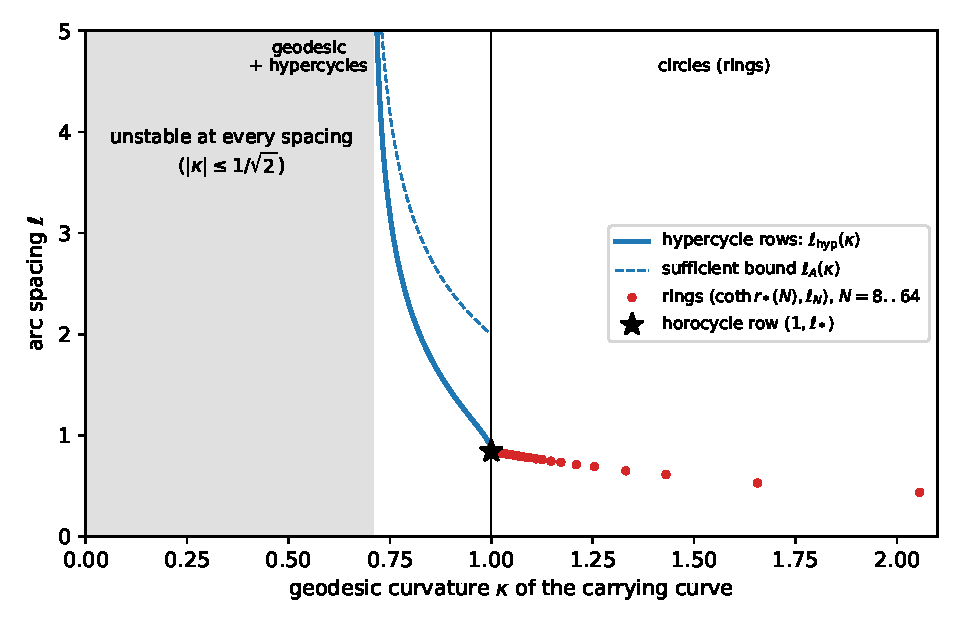
\includegraphics[width=0.86\textwidth]{figures/boundary.pdf}
\caption{Stability boundary of equally spaced vortex arrays on $\HH$ (tanh model) in the plane of geodesic curvature $\kappa$
of the carrying curve and arc spacing $\ell$. Grey: unstable at every spacing (Theorem~\ref{thm:kappac}). Blue: hypercycle
threshold $\ell_{\rm hyp}(\kappa)$ (Theorem~\ref{thm:single}); dashed: the explicit sufficient bound $\ell_A(\kappa)$. Star: the
horocycle row (Theorem~\ref{thm:row}). Red: threshold rings $(\coth r_*(N),\ell_N)$, $N=8,\dots,64$. Arrays above the curve are
spectrally stable. Plotted values are floating point (\nolinkurl{code/make_figures.py}).}\label{fig:boundary}
\end{figure}

\paragraph{Why curvature stabilises.} The planar row is unstable at every spacing, and so is a row along a geodesic of $\HH$,
although it has the same screened interaction (Theorem~\ref{thm:kappac}(a)). What stabilises sparse horocycle and hypercycle
rows is the bending of the carrying curve: the critical curvature $1/\sqrt2$ is where, at large spacing, the stiffness that
the curvature gives the pairing mode balances the attraction of a vortex to its displaced neighbours (Remark~\ref{rem:45}).
For rings the same mechanism appears as a critical \emph{spacing}: a large ring is stable once neighbours are more than
$\ell_*\approx0.844$ curvature radii apart.

\paragraph{Status labels.} Every claim carries one label. \st{Lean}: checked in Lean~4 with Mathlib \cite{Mathlib2020};
we name the theorem in the library \texttt{HyperbolicRings} (directory \texttt{lean/}). \st{Proved}: proof by hand in this
paper. \st{Certified}: exact rational or interval (Arb \cite{Johansson2017}) arithmetic, with script and output named.
\st{Derived}: formal asymptotics. \st{Numerical}: floating-point evidence. Where a Lean statement rests on a modelling input that is not
itself formalised (Hamilton's equations in a chart, the identification of the linearisation of an infinite row with a lattice sum of
pair terms) we say so. The file \texttt{README.md} next to the paper maps every numbered statement to its proof, Lean theorem, script and
output.

%======================================================================
\section{Setting}\label{sec:setting}

\subsection{Hamiltonian and stability notions}
In the Poincar\'e disk $\D$ with metric $4|dz|^2/(1-|z|^2)^2$ we have $\tanh(d(z,w)/2)=|z-w|/|1-z\bar w|$, so
\begin{equation}\label{eq:H}
H=\sum_{j<k}\Big(-\log|z_j-z_k|+\log|1-z_j\bar z_k|\Big),\qquad
\omega=\sum_k\frac{4\,dx_k\wedge dy_k}{(1-|z_k|^2)^2},\qquad J=\sum_k\cosh r_k,
\end{equation}
where $J$ generates the rotations about $0$. (The function $f(d)=\log\tanh(d/2)$ satisfies $f''+\coth d\,f'=0$, so $G$ is the
Green function; the pair term in~\eqref{eq:H} is also the Green function of the flat unit disk with a conducting wall, but the
symplectic form differs.) The full symmetry group is the isometry group $PSL(2,\mathbb R)$.

A configuration $x_0$ is a \emph{relative equilibrium} if it is a critical point of $F=H-\Omega J$ for some $\Omega$ (here
$J$ is the momentum of a one-parameter subgroup: rotations for rings, the translations along the curve for rows). The
linearised flow at $x_0$ is $\mathcal L=\omega^{-1}d^2F(x_0)$.
\begin{definition}\label{def:stab}
$x_0$ is \emph{spectrally stable} if every eigenvalue of $\mathcal L$ has zero real part. It is \emph{definite} (on a given
invariant subspace $V$) if $d^2F(x_0)|_V$ is positive definite. For a ring, $V$ is the sum of the Fourier modes
$m=1,\dots,N-1$ (all but the rotation/dilation mode $m=0$). For an infinite row, stability and definiteness are imposed on each
Bloch wave $q\in(0,2\pi)$.
\end{definition}
Definiteness on $V$ is the hypothesis of the energy--momentum method \cite{SimoLewisMarsden1991}; it implies spectral stability
on $V$ but not conversely. When $d^2F|_V$ is indefinite and the spectrum is imaginary, the eigenvalues carry \emph{Krein
signatures} (the sign of $d^2F$ on the eigenvector) \cite{MacKay1986}: an eigenvalue pair of opposite signatures can
collide and leave the imaginary axis under perturbation, and nonlinear stability is not decided by the quadratic form. We
claim nonlinear stability nowhere in this paper. (Positive definiteness on $V$ yields Lyapunov stability only modulo the
symmetry group; the modes $m=\pm1$ are tangent to the non-compact boost directions of $PSL(2,\mathbb R)$, and we have not
verified the hypotheses of a specific energy--momentum theorem for this model.)

\subsection{The ring}
Let $w=e^{2\pi i/N}$ and $z_j=\sqrt\xi\,w^je^{s_j+i\theta_j}$, so the ring of Euclidean radius $\sqrt\xi$ is $s=\theta=0$. Then
$\omega=\sum_j\rho(s_j)\,ds_j\wedge d\theta_j$ with $\rho_0:=\rho(0)=4\xi/(1-\xi)^2=\sinh^2r$. Put
\[
c:=\cosh r=\frac{1+\xi}{1-\xi},\qquad X:=\xi^N,\qquad W_k:=\sum_{\substack{p\ge1\\p\equiv k\ (N)}}p\,\xi^p=\frac{k\xi^k}{1-X}+\frac{N\xi^{k+N}}{(1-X)^2}\quad(1\le k\le N).
\]
\begin{lemma}[relative equilibrium; \st{Lean}]\label{lem:re}
For every $N\ge1$ and $\xi\in(0,1)$ the ring is a critical point of $F=H-\Omega J$ in all $2N$ variables exactly when
$\Omega\rho_0=-\frac{N-1}2+\frac{\xi}{1-\xi}-\frac{NX}{1-X}$.
Lean: \lean{HyperbolicRings.Tanh.ring_critical} (with \lean{ring_critical_iff}).
\end{lemma}
The proof uses the power-sum expansion $\log|1-u|=-\operatorname{Re}\sum_{p\ge1}u^p/p$, which turns~\eqref{eq:H} into
\begin{equation}\label{eq:decomp}
H=-\sum_{j<k}\log|z_j-z_k|-\frac12\sum_j\log(1-|z_j|^2)-\frac12\sum_{p\ge1}\frac{|P_p|^2}p,\qquad P_p=\sum_jz_j^p;
\end{equation}
on a ring the last term is diagonal in the Fourier modes. The $\theta$-derivatives vanish by symmetry; the $s_j$-derivatives
give the stated $\Omega$. (Appendix~\ref{app:blocks} gives the computation; Lean derives it from the Hamiltonian.)

%======================================================================
\section{Fourier blocks and the ring threshold}\label{sec:blocks}

\begin{theorem}[Fourier blocks; \st{Lean}]\label{thm:blocks}
At the ring, $d^2F$ is block-circulant in $(s,\theta)$. On the Fourier mode $(s_j,\theta_j)=(S,T)w^{mj}$, $1\le m\le N-1$, it
acts as the Hermitian matrix $M_m=\begin{psmallmatrix}a_m&ig_m\\-ig_m&b_m\end{psmallmatrix}$, where
\begin{align*}
a_m&=(N-1)c-\tfrac12(c-1)^2-\tfrac{m(N-m)}2+\frac{2NcX}{1-X}-NW_N-\tfrac N2\,(W_m+W_{N-m}),\\
b_m&=\tfrac{m(N-m)}2+NW_N-\tfrac N2\,(W_m+W_{N-m}),\qquad g_m=\tfrac N2\,(W_m-W_{N-m}).
\end{align*}
All entries are rational functions of $\xi$ with rational coefficients; $a_{N-m}=a_m$, $b_{N-m}=b_m$, $g_{N-m}=-g_m$, and
$g_{N/2}=0$ for even $N$. Lean: \lean{HyperbolicRings.Tanh.blocks_eigen} (the Hessian, computed from $H$ as explicit
circulant matrices in \lean{BlocksHess}, acts on $(w^{mb})_b$ by $a_m,b_m,g_m$), \lean{blocks_hermitian}.
\end{theorem}
Here $a_m$ is the radial and $b_m$ the tangential stiffness of mode $m$, and $g_m$ is a radial--tangential coupling which has
no analogue in the planar or sinh-model ring. The hand proof is in Appendix~\ref{app:blocks}. Under $\xi\mapsto1/\xi$ the
entries satisfy $a_m\mapsto a_m$, $b_m\mapsto b_m$, $g_m\mapsto-g_m$ (inversion in the boundary circle), so the cleared
numerators are self-reciprocal polynomials; we use this only as a check.

\begin{proposition}[linearisation; \st{Lean}]\label{prop:lin}
On mode $m$ the linearised flow is $\rho_0(\dot S,\dot T)^{\top}=J_0M_m(S,T)^{\top}$, $J_0=\begin{psmallmatrix}0&1\\-1&0\end{psmallmatrix}$, with
eigenvalues $\rho_0\lambda=-ig_m\pm\sqrt{-a_mb_m}$; the spectrum of $\mathcal L$ on $\mathbb R^{2N}$ is the union over $m$. Hence the
ring is spectrally stable iff $a_mb_m\ge0$ for all $1\le m\le N-1$, and definite on $V$ iff $a_m>0$ and $a_mb_m-g_m^2>0$ for all
such $m$. Lean: \lean{linFlow_spectral_iff}, \lean{hessQ_posDef_compl_iff} (module \lean{Tanh.LinearFlow}), \lean{flowBlock_hasEigenvalue_iff},
\lean{specStable_iff_spectral}.
\end{proposition}
\begin{proof}
$\det(J_0M_m-\lambda)=(\lambda+ig_m)^2+a_mb_m$; a Hermitian $2\times2$ matrix is positive definite iff its $(1,1)$ entry and its
determinant are positive. Distinct modes are $d^2F$- and $\omega$-orthogonal.
\end{proof}
So $g_m$ shifts the frequencies but does not affect spectral stability; it does affect definiteness (\S\ref{sec:krein}).

\subsection{The exact symbol}
Put $\tau:=-\frac N2\log\xi\in(0,\infty)$, so that $\xi^N=e^{-2\tau}$ and $\cosh r=\coth(\tau/N)$ ($\tau\to0$ as $r\to\infty$), and
for $1\le m\le N-1$ put $x:=1-2m/N\in(-1,1)$. Let
\[
Q(x,\tau)=\cosh\tau\cosh x\tau-x\sinh\tau\sinh x\tau,\qquad R(x,\tau)=\cosh\tau\sinh x\tau-x\sinh\tau\cosh x\tau,
\]
\[
\beta=\frac{1-x^2}8+\frac{1-Q}{4\sinh^2\tau},\qquad \psi=\frac{1-x^2}8+\frac{Q}{4\sinh^2\tau},\qquad \gamma=\frac{R}{4\sinh^2\tau},
\]
\[
E_N(\tau)=k\coth\tau-\frac{k^2}2-\frac1{2N^2},\qquad k=\frac{\coth(\tau/N)}N .
\]
\begin{theorem}[exact symbol; \st{Lean}]\label{thm:symbol}
For every $N\ge2$, $1\le m\le N-1$ and $\xi\in(0,1)$,
\[
\frac{a_m}{N^2}=E_N(\tau)-\frac1{4\sinh^2\tau}-\psi(x,\tau),\qquad \frac{b_m}{N^2}=\beta(x,\tau),\qquad \frac{g_m}{N^2}=\gamma(x,\tau).
\]
Lean: \lean{aBlock_xiOf}, \lean{bBlock_xiOf}, \lean{gBlock_xiOf}.
\end{theorem}
\begin{proof}
With $\xi^j=e^{-2j\tau/N}$: $\xi^m=e^{-(1-x)\tau}$, $1-X=2e^{-\tau}\sinh\tau$, and from the closed form of $W_k$,
$(W_m+W_{N-m})/N=Q/(2\sinh^2\tau)$, $(W_m-W_{N-m})/N=2\gamma$, $NW_N=N^2/(4\sinh^2\tau)$ (use $\sinh\tau+e^{-\tau}=\cosh\tau$). For
$a_m$ note that the one-body part equals $Nc\coth\tau-\frac{c^2}2-\frac12$ and $m(N-m)=N^2(1-x^2)/4$.
\end{proof}
The mode number enters only through $x$, and in $a_m$ only through $\psi$: up to an $m$-independent term the blocks are a
function of $m/N$. This is what makes all $N$ tractable at once.

\begin{lemma}[tangential stiffness; \st{Lean}]\label{lem:bpos}
$\beta(x,\tau)>0$ for $|x|<1$, $\tau>0$; hence $b_m>0$ for every $N\ge2$, $1\le m\le N-1$, $\xi\in(0,1)$.
Lean: \lean{beta_pos}, \lean{bBlock_pos}.
\end{lemma}
\begin{proof}
With $a=(1+x)\tau$, $b=(1-x)\tau$ and $f(t)=\sinh^2(t/2)/t$ one checks $\beta=\frac{ab}{4\tau\sinh^2\tau}[f(a+b)-f(a)-f(b)]$. Since
$f(t)/t$ is strictly increasing, $f$ is strictly superadditive on $(0,\infty)$.
\end{proof}

\begin{lemma}[critical mode; \st{Lean}]\label{lem:crit}
For every $\tau>0$, $\psi(\cdot,\tau)$ is even and strictly decreasing on $[0,1]$. Hence $a_m\ge a_{\lfloor N/2\rfloor}$, with
equality only for $m\in\{\lfloor N/2\rfloor,\lceil N/2\rceil\}$, and the ring is spectrally stable iff
$a_{\lfloor N/2\rfloor}\ge0$; if $a_{\lfloor N/2\rfloor}<0$ the modes $\lfloor N/2\rfloor,\lceil N/2\rceil$ grow exponentially.
Lean: \lean{psi_strictAntiOn}, \lean{aBlock_half_le}, \lean{aBlock_half_lt}, \lean{specStable_iff}.
\end{lemma}
The proof (a careful but elementary estimate of $\partial_x\psi$ through $\lambda(t)=\log(\sinh t/t)$) is in
Appendix~\ref{app:crit}.

\subsection{\texorpdfstring{One threshold for every $N\ge8$}{One threshold for every N >= 8}}
\begin{theorem}[\st{Lean}]\label{thm:unique}
\begin{enumerate}
\item[(a)] For $2\le N\le7$ and every $\xi\in(0,1)$: $a_m>0$, $b_m>0$ and $a_mb_m-g_m^2>0$ for all $m$. The ring is spectrally
stable and definite on $V$ at every radius.
\item[(b)] For every $N\ge8$ there is $\xi_*(N)\in(0,1)$ such that $a_{\lfloor N/2\rfloor}<0$ on $(0,\xi_*)$, $=0$ at $\xi_*$ and $>0$
on $(\xi_*,1)$. The ring is spectrally unstable for $\xi<\xi_*$ (in the modes $\lfloor N/2\rfloor$, $\lceil N/2\rceil$) and
spectrally stable for $\xi\ge\xi_*$.
\item[(c)] $\xi_*(N)$ is algebraic: it is a root of the integer polynomial $2(1-\xi)^2(1-\xi^N)^2a_{\lfloor N/2\rfloor}$.
\end{enumerate}
Lean: (a) \lean{stable_N2}, \dots, \lean{stable_N7}, \lean{stable_all_radii_of_le_seven}; (b)
\lean{unique_threshold_of_ge_eight}; (c) is immediate from Theorem~\ref{thm:blocks}.
\end{theorem}
\begin{proof}
Spectral stability is equivalent to $a_{\lfloor N/2\rfloor}\ge0$ (Lemma~\ref{lem:crit}). The proof of (b) splits by parity.

\emph{Even $N$.} At $x=0$ and with $\eta=\tau/2$, $\mu=\frac2N\coth\frac{2\eta}N$, Theorem~\ref{thm:symbol} gives
\begin{equation}\label{eq:even}
\frac{8a_{N/2}}{N^2}=2\mu\tanh\eta-(\coth\eta-\mu)^2-\frac4{N^2}.
\end{equation}
For $N\ge4$ this is strictly decreasing in $\eta$: $\mu\tanh\eta=\frac2N\tanh(qv)/\tanh v$ with $v=2\eta/N$, $q=N/2>1$, has
logarithmic derivative $\frac{2q}{\sinh2qv}-\frac2{\sinh2v}<0$, and $\coth\eta-\mu\ge0$ is non-decreasing, both because
$t/\sinh t$ decreases. The limits are $2-4/N^2$ as $r\to\infty$ and the planar value $-(N^2-8N+8)/N^2$ as $r\to0$, which is
negative iff $N\ge8$ (Lean: \lean{aBlock_half_threshold}, \lean{aBlock_half_pos_of_le_six}).

\emph{Odd $N\ge17$.} Here $a_{(N-1)/2}/N^2=\Phi_N(\tau)+\varepsilon_N(\tau)$, where $\Phi_N$ is the right side of~\eqref{eq:even}
divided by $8$ (strictly decreasing by the same argument) and $\varepsilon_N=\psi(0,\tau)-\psi(1/N,\tau)\in[0,1/(4N^2)]$.
Explicit bounds on $\Phi_N$, $\varepsilon_N$ and their $\tau$-derivatives show that $a_{(N-1)/2}$ is positive for $\tau\le5$,
negative for $\tau\ge10$ and strictly decreasing on $[5,10]$ (Lean: \lean{aBlock_half_threshold_of_ge_17}; the estimates
are in \lean{Tanh.LargeN.OddN}).

\emph{Odd $9\le N\le15$ and all $N\le7$.} Exact computation: for each $N$ and $m$ the cleared numerators of $a_m$, $b_m$ and
$a_mb_m-g_m^2$ are explicit integer polynomials, and their sign pattern on $(0,1)$ is proved in Lean by polynomial
positivity certificates and a rational isolating interval for the root of $a_{\lfloor N/2\rfloor}$
(\lean{cert_N9}, \lean{cert_N11}, \lean{cert_N13}, \lean{cert_N15}, \lean{stable_N2}--\lean{stable_N7}; independently by exact
real-root isolation in \nolinkurl{code/tanh_threshold_polys.py}).
\end{proof}

\begin{table}[t]\centering\small
\begin{tabular}{rlllrr}\toprule
$N$ & $\xi_*(N)$ & $r_*(N)$ & $\cosh r_*(N)$ & $\deg$ & $\xi_{\rm EM}-\xi_*$\\\midrule
8 & 0.0673562230040812622684374\ldots & 0.5312104560 & 1.1444414784 & 10 & 0\\
9 & 0.1128710632366027404396940\ldots & 0.6990695396 & 1.2544637167 & 16 & $3.220\cdot10^{-8}$\\
10 & 0.1661142415262391180817586\ldots & 0.8653901256 & 1.3984100696 & 12 & 0\\
11 & 0.2046011768826692906355358\ldots & 0.9752480466 & 1.5144618547 & 20 & $1.244\cdot10^{-7}$\\
12 & 0.2474177768040677091739650\ldots & 1.0917203545 & 1.6575169309 & 16 & 0\\
13 & 0.2798613886439066870299965\ldots & 1.1775646302 & 1.7772431147 & 24 & $1.777\cdot10^{-7}$\\
14 & 0.3149389631155066233935054\ldots & 1.2691494599 & 1.9194478920 & 18 & 0\\
15 & 0.3424585835121702566010226\ldots & 1.3406681986 & 2.0416335000 & 28 & $1.886\cdot10^{-7}$\\
16 & 0.3716818139060454566367287\ldots & 1.4167509599 & 2.1831006077 & 22 & 0\\\bottomrule
\end{tabular}
\caption{Ring thresholds, $8\le N\le16$. \st{Certified}: $\xi_*(N)$ lies in an exact rational interval of width $<10^{-45}$
on which the cleared critical numerator changes sign, and in an Arb ball of radius $<3\cdot10^{-153}$
(\nolinkurl{code/tanh_threshold_polys.py}); Lean locates it in a rational interval of width $10^{-20}$ (\lean{cert_N8},
\dots, \lean{cert_N16}). $r_*$ and $\cosh r_*$ are evaluated from $\xi_*$. ``deg'' is the degree of the minimal polynomial
of $\xi_*$: the factor $f_N$ of the critical numerator carrying $\xi_*$ is irreducible over $\mathbb Q$ (Lean:
\lean{f8_irreducible}, \dots, \lean{f16_irreducible}, by mod-$p$ certificates), and palindromic. Last column: the Krein
window (Theorem~\ref{thm:krein}; \st{Certified}, \nolinkurl{code/tanh_krein.py}).}\label{tab:thr}
\end{table}

\begin{remark}[algebraic structure; \st{Certified}/\st{Lean}]\label{rem:alg}
That $\xi_*(N)$ is algebraic is automatic from Theorem~\ref{thm:blocks}; the structure is not. For $8\le N\le16$ the minimal
polynomial is palindromic (so $1/\xi_*$ is a Galois conjugate, the image of the ring under inversion in the boundary circle) of
degree $2N-2$ for odd $N$, $\frac32N-2$ for $N\equiv0$, and $\frac32N-3$ for $N\equiv2\pmod4$; $\xi_*(8)$ is a unit with minimal
polynomial $x^{10}-12x^9-37x^8-72x^7-84x^6-88x^5-84x^4-72x^3-37x^2-12x+1$, while for $9\le N\le16$ the leading coefficient
exceeds $1$ and $\xi_*(N)$ is not an algebraic integer. Irreducibility is in Lean; the degree pattern for general $N$ is open.
\end{remark}

\begin{remark}[comparison with Boatto; \st{Numerical}]\label{rem:boatto}
Boatto \cite{Boatto2008} fixes the geodesic radius $r_0=1$ and varies the curvature $K_{\rm B}<0$; then
$\xi=\tanh^2(\sqrt{-K_{\rm B}}/2)$. Implementing her Hessian (her eqs.~(14), (17), (29), (31); equation numbers as in the journal
version) independently of our blocks, the zero crossing of her determinant for $N=8$ is $K_{\rm B}=-0.28218454857650183188$, which maps to $\xi_*(8)$ to $10^{-41}$; for $N=10$ the agreement is $10^{-42}$.
For $N=9$ her (definiteness) criterion gives $\xi_{\rm EM}(9)$, i.e.\ $\xi_*(9)+3.22\cdot10^{-8}$, as it must by
Theorem~\ref{thm:krein}. Her mode blocks are ours up to $m$-independent positive factors
(\nolinkurl{code/boatto_map_and_verify.py}).
\end{remark}

%======================================================================
\section{\texorpdfstring{Odd $N$}{Odd N}: the Krein window}\label{sec:krein}

Let $\xi_{\rm EM}(N)=\inf\{\xi_0:\ d^2F$ is definite on $V$ for all $\xi\in(\xi_0,1)\}$. Since definiteness implies spectral
stability, $\xi_{\rm EM}\ge\xi_*$.

\begin{lemma}[definiteness excess; \st{Lean}]\label{lem:em}
Let $\Phi_N(\tau)=E_N(\tau)-\frac1{4\sinh^2\tau}-\psi(0,\tau)$ and $\mathcal G=\psi(0,\tau)-\psi(x,\tau)-\gamma^2/\beta$. Then
$\mathcal G\ge0$, with equality only at $x=0$, and $a_mb_m-g_m^2=N^4\beta\,[\Phi_N(\tau)+\mathcal G(x,\tau)]$.
Lean: \lean{beta_mul_G}, \lean{K_pos}, \lean{G_nonneg}, \lean{det_xiOf}.
\end{lemma}
\begin{proof}
With $C=\cosh\tau$, $S=\sinh^2\tau$: $8SB\mathcal G=AB-4R^2$, where $A=x^2S+2C-2Q$ and $B=8S\beta$; using $Q^2-R^2=C^2-x^2S$ this
equals $2(C+1)^2\mathcal K$ with
$\mathcal K=C(1-\cosh x\tau)+x\sinh\tau\sinh x\tau-\frac{x^2(C-1)}2[2-(1-x^2)(C-1)]$. Now $\mathcal K(x,0)=0$ and
$\partial_\tau\mathcal K=\sinh\tau(1-x^2)[x^2(C-1)-(\cosh x\tau-1)]>0$ for $0<|x|<1$.
\end{proof}

\begin{theorem}[Krein window]\label{thm:krein}
\begin{enumerate}
\item[(a)] \st{Lean} For even $N$ and every radius, $d^2F$ is definite on $V$ iff $a_{N/2}>0$; hence $\xi_{\rm EM}(N)=\xi_*(N)$
and there is no window. (\lean{emDefinite_iff_even}, \lean{xiEM_eq_xiStar_even}.)
\item[(b)] \st{Lean} For every odd $N\ge9$: $0<\xi_*<\xi_{\rm EM}<1$; the ring is spectrally stable on $(\xi_*,1)$; and there is
$\eta>0$ with $a_mb_m-g_m^2<0$ for $m=\frac{N-1}2$ on $(\xi_*,\xi_*+\eta)$. Moreover $\xi_{\rm EM}-\xi_*=O(N^{-3})$.
(\lean{krein_window_odd}, \lean{HyperbolicRings.Krein.krein_window_bounds}, \lean{xiEM_lt_one},
\lean{xiEM_sub_xiStar_le}.)
\item[(c)] \st{Lean} On that interval the critical mode has two distinct purely imaginary eigenvalues
$\rho_0\lambda_\pm=i(-g_m\pm\sqrt{a_mb_m})$, and the quadratic form $d^2F$ has opposite signs on their eigenvectors (opposite
Krein signatures). (\lean{HyperbolicRings.Krein.ring_window_hypotheses}, \lean{opposite_signatures},
\lean{eigenvalues_imaginary_distinct}.)
\item[(d)] \st{Certified} For $N=9,11,13,15$ the window $(\xi_*,\xi_{\rm EM})$ is given in Table~\ref{tab:thr} (disjoint exact
rational isolating intervals), and on the whole window the critical block is indefinite while every other block is positive
definite (\nolinkurl{code/tanh_krein.py}). For $N\in\{17,21,31,61,121,241\}$ the same holds at sampled points \st{Numerical}
(\nolinkurl{code/tanh_extras.py}).
\end{enumerate}
\end{theorem}
\begin{proof}
(a) By Lemma~\ref{lem:crit}, $a_m\ge a_{N/2}=N^2\Phi_N$; if $\Phi_N>0$ Lemma~\ref{lem:em} gives $a_mb_m-g_m^2>0$ for all $m$.

(b) The planar limit $-(N-1)(N-7)/N^2<0$ of $8a_{(N-1)/2}/N^2$ gives $\xi_*>0$. At $\xi_*$, $a_mb_m-g_m^2=-g_m^2<0$ because
$R(1/N,\tau)>0$ ($\tanh$ is strictly concave on $[0,\infty)$, so $\tanh x\tau>x\tanh\tau$); continuity gives $\eta$. For the
width: $\Phi_N>0$ implies definiteness (Lemma~\ref{lem:em}), $\Phi_N$ has slope bounded away from $0$ near $\tau_\infty$ (\S\ref{sec:largeN}),
and $a_{(N-1)/2}/N^2-\Phi_N=\varepsilon_N=O(N^{-2})$; so the two $\tau$-thresholds differ by $O(N^{-2})$, and $\xi=e^{-2\tau/N}$
gives a further factor $2/N$.

(c) $a_mb_m>0$ on the interval, since $a_m>0$ above $\xi_*$ (Theorem~\ref{thm:unique}) and $b_m>0$. For
$M=\begin{psmallmatrix}a&ig\\-ig&b\end{psmallmatrix}$ and $\mu=\pm\sqrt{ab}$, every eigenvector of $J_0M$ for $i(-g+\mu)$ is a
multiple of $(b,i\mu)$, and $(b,i\mu)^*M(b,i\mu)=2b\mu(\mu-g)$. The product of the two values is $4b^2\,ab\,(ab-g^2)<0$.
\end{proof}

\paragraph{What the window means.} Throughout $(\xi_*,\xi_{\rm EM})$ the odd ring is spectrally stable, with semisimple
spectrum on $V$ (the rotation mode $m=0$ carries a Jordan block whenever $c_0\neq0$; numerically $c_0>0$ for every $N$ checked), but no Lyapunov function of energy--momentum type exists, and the two critical frequencies, of opposite
signature, may collide under a perturbation (for example, a change of the model) and produce a Hamiltonian--Hopf instability.
Whether the ring is nonlinearly stable inside the window is open. A criterion based on definiteness of the Hessian, such as the
one used in \cite{Boatto2008}, reports the threshold $\xi_{\rm EM}$ and so misses the window; for $N\le15$ the difference is
below $2\cdot10^{-7}$ in $\xi$. Expanding the critical block suggests $N^3(\xi_{\rm EM}-\xi_*)\to0.003709\ldots$ \st{Derived}
(assuming the critical block is the last to become definite); the data give $0.00348$ at $N=241$.

%======================================================================
\section{\texorpdfstring{Large $N$}{Large N} and the horocycle row}\label{sec:largeN}

\subsection{The limit function}
As $N\to\infty$ at fixed $\tau$, $E_N\to\coth\tau/\tau-1/(2\tau^2)$ and the critical block tends to
$a_{\lfloor N/2\rfloor}/N^2\to\Phi(\tau)$, with
\begin{equation}\label{eq:Phi}
8\,\Phi(\tau)=\frac4\tau\tanh\frac\tau2-\Lan\Big(\frac\tau2\Big)^2,\qquad \Lan(\eta)=\coth\eta-\frac1\eta .
\end{equation}
\begin{lemma}[\st{Lean}; digits \st{Certified}]\label{lem:Phi}
$\Phi$ is strictly decreasing on $(0,\infty)$ from $\frac14$ to $-\frac18$; its unique zero $\tau_\infty$ satisfies
$7.4453<\tau_\infty<7.4454$ (Lean: \lean{Phi_strictAntiOn}, \lean{existsUnique_Phi_zero}, \lean{tauInf_bracket}). An Arb
bracket gives
\[
\tau_\infty\in(7.4453392449490186871,\,7.4453392449490186873),
\]
so $\ell_*:=2\pi/\tau_\infty=0.84390853129253347\ldots$ and
$\Phi'(\tau_\infty)=-0.01532424264\ldots$ (\nolinkurl{code/tanh_large_n.py}).
\end{lemma}
\begin{proof}
$(\tanh\eta/\eta)'<0$ and $(\Lan^2)'=2\Lan\Lan'>0$. The bracket is a sign evaluation with explicit bounds for $\exp$.
\end{proof}
Dropping the exponentially small terms turns $\Phi(\tau_\infty)=0$ into $\eta^2-4\eta+1=0$ for $\eta=\tau/2$; so
$\tau_\infty/2\approx2+\sqrt3$ and $\ell_*\approx\pi(2-\sqrt3)=0.8418$ \st{Numerical}.

\begin{theorem}[large-$N$ threshold; \st{Lean}]\label{thm:largeN}
For both parities of $N$,
\[
\cosh r_*(N)=\frac N{\tau_\infty}+O\Big(\frac1N\Big),\qquad \ell_N:=\frac{2\pi\sinh r_*(N)}N=\ell_*+O(N^{-2}),
\]
and the same holds for $\xi_{\rm EM}(N)$. Lean: \lean{cR_xiStar_rate}, \lean{tendsto_cR_xiStar}, \lean{spacing_rate},
\lean{cR_xiEM_rate}.
\end{theorem}
\begin{proof}
By Theorem~\ref{thm:symbol}, $a_{\lfloor N/2\rfloor}/N^2=\Phi(\tau)+\Delta_N(\tau)+\varepsilon_N(\tau)$ with
$\Delta_N=E_N-E_\infty$ and $\varepsilon_N=\psi(0,\tau)-\psi(x_N,\tau)$, $x_N\in\{0,1/N\}$. Writing $\delta=\Lan(\tau/N)/N$ one finds
$-\frac1{2N^2}-\frac{\delta^2}2\le\Delta_N\le\frac\tau{3N^2}$, and $0\le\varepsilon_N\le1/(4N^2)$. Since $\Phi'(\tau_\infty)\ne0$,
$a_{\lfloor N/2\rfloor}$ is positive at $\tau_\infty-K/N^2$ and negative at $\tau_\infty+K/N^2$ for large $K$, so
$|\tau_*(N)-\tau_\infty|\le K/N^2$ by uniqueness of the threshold. Finally $\cosh r_*=\coth(\tau_*/N)$ and
$\sinh r_*=1/\sinh(\tau_*/N)$.
\end{proof}
So at threshold the neighbours of a large ring are $\ell_*\approx0.844$ curvature radii apart along the ring (geodesic distance
$2\operatorname{arsinh}(\ell_*/2)=0.82068\ldots$). In the sinh model, by contrast, $\cosh r_*\sim\sqrt N/2$ and the threshold
spacing tends to $0$ \cite{MontaldiTokieda2013}.

\begin{proposition}[second order; \st{Proved}, constants \st{Numerical}]\label{prop:second}
For each parity there is $N_0$ such that for $N\ge N_0$ the quantities $\tau_*(N)$, $\cosh r_*(N)/N$ and $\ell_N$ are values at
$N^{-2}$ of real-analytic functions, and
\[
\cosh r_*(N)=\frac N{\tau_\infty}+\frac{\varsigma}N+O(N^{-3}),\qquad \ell_N=\ell_*+\frac{2\pi(\varsigma-\tau_\infty/2)}{N^2}+O(N^{-4}),
\]
\[
\varsigma=\frac{\tau_\infty}3-\frac{\mathcal D+[N\text{ odd}]\,p(\tau_\infty)}{|\Phi'(\tau_\infty)|\,\tau_\infty^2},\qquad
\mathcal D=\frac{\tau_\infty\coth\tau_\infty-1}3-\frac12,\qquad p(\tau)=-\tfrac12\,\partial_x^2\psi(0,\tau).
\]
Numerically $\varsigma_{\rm e}=0.5412188400$, $\varsigma_{\rm o}=0.4010382403$, $\ell_N-\ell_*\approx-19.990N^{-2}$ (even) and
$-20.870N^{-2}$ (odd); the thresholds give $N(\cosh r_*-N/\tau_\infty)=0.5412206$ at $N=800$ and $0.4010393$ at $N=801$
(\nolinkurl{code/b4_varsigma.py}, \nolinkurl{code/tanh_large_n.py}; Figure~\ref{fig:largeN}).
\end{proposition}
\begin{proof}
With $\epsilon=N^{-2}$ and $y=\tau/N$, $k=(y\coth y)/\tau$ is an even analytic function of $y$, hence analytic in
$(\tau,\epsilon)$ ($y^2=\tau^2\epsilon$), and $\psi(x,\tau)$ is even in $x$, so $\psi(1/N,\tau)$ is analytic in $\epsilon$. Thus
$a_{\lfloor N/2\rfloor}/N^2=\Psi_{\rm par}(\tau,\epsilon)$ with $\Psi_{\rm par}$ analytic near $(\tau_\infty,0)$ and
$\Psi_{\rm par}(\tau,0)=\Phi(\tau)$. Since $\Phi'(\tau_\infty)\neq0$ the implicit function theorem gives an analytic zero
$\tau(\epsilon)$, which is $\tau_*(N)$ by Theorem~\ref{thm:largeN} and uniqueness. Expanding $y\coth y=1+y^2/3+\dots$ gives
$\partial_\epsilon\Psi_{\rm par}(\tau,0)=\mathcal D(\tau)+[N\text{ odd}]p(\tau)$, so $\tau_*=\tau_\infty+\epsilon(\mathcal D+[\text{odd}]p)/|\Phi'|+O(\epsilon^2)$;
then $\cosh r_*=\coth(\tau_*/N)=N/\tau_*+\tau_*/(3N)+O(N^{-3})$ and $\ell_N=2\pi/(N\sinh(\tau_*/N))=2\pi/\tau_*-2\pi\tau_*/(6N^2)+O(N^{-4})$.
\end{proof}
Lean computes $\partial_x^2\psi(0,\tau)=-\frac14+\frac{\tau^2\cosh\tau-2\tau\sinh\tau}{4\sinh^2\tau}$ and proves that it is
negative at $\tau_\infty$, so $p(\tau_\infty)>0$ and $\varsigma_{\rm o}<\varsigma_{\rm e}$
(\lean{HyperbolicRings.Horocycle.second_deriv_psi}, \lean{psiXX_tauInf_neg}); the implicit-function step is not in Lean.

\begin{figure}[t]\centering
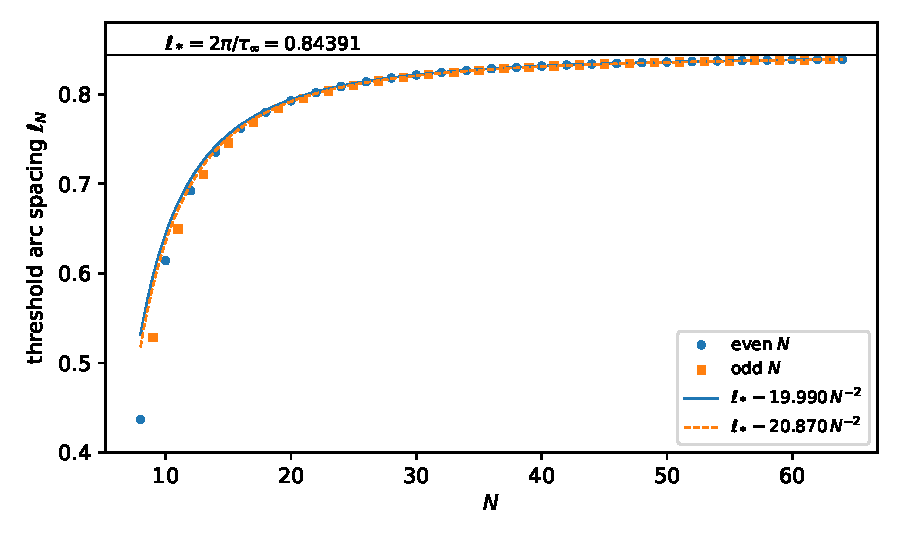
\includegraphics[width=0.74\textwidth]{figures/large_n.pdf}
\caption{Threshold arc spacing $\ell_N=2\pi\sinh r_*(N)/N$ of the $N$-ring against $N$, with the limit $\ell_*$ (Theorem~\ref{thm:largeN})
and the second-order curves of Proposition~\ref{prop:second} for each parity. Floating point.}\label{fig:largeN}
\end{figure}

\subsection{The horocycle row}
In the upper half-plane (metric $|dz|^2/y^2$) the pair term is $-\log\tanh(d/2)=-\log|z-w|+\log|z-\bar w|$: a planar row plus
its mirror image, with the hyperbolic symplectic form $dx\wedge dy/y^2$. Take the horocycle $y=1$ and the row $z_k=k\ell+i$,
$k\in\mathbb Z$. The translations $x\mapsto x+t$ are isometries with momentum $J=-\sum_k1/y_k$. The forces on a vortex converge
absolutely (the pair and image terms together decay like $k^{-3}$ and $k^{-2}$), and the Hessian couples sites through
absolutely summable $2\times2$ blocks, so on a Bloch wave $(\delta x_k,\delta y_k)=e^{2\pi i\theta k}(\delta x,\delta y)$ it
acts by a Hermitian matrix $M(\theta)$.

\begin{theorem}[horocycle row; \st{Lean}]\label{thm:row}
Let $\tau=2\pi/\ell$ and $x=1-2\theta$.
\begin{enumerate}
\item[(a)] The row is a relative equilibrium drifting at $\dot x=\frac12(\tau\coth\tau-1)$, and, in the basis $(\delta x,\delta y)$,
\[
\Big(\frac\ell{2\pi}\Big)^2M(\theta)=\begin{pmatrix}\beta&i\gamma\\-i\gamma&\mathfrak a\end{pmatrix}(x,\tau),\qquad
\mathfrak a=\frac{\coth\tau}\tau-\frac1{2\tau^2}-\frac1{4\sinh^2\tau}-\psi(x,\tau),
\]
with $\beta,\gamma,\psi$ as in Theorem~\ref{thm:symbol}. So the ring blocks divided by $N^2$ converge, at fixed $(m/N,\tau)$, to
the row symbol, with ring mode number $m/N$ becoming the Bloch number $\theta$ and the ring's (tangential, outward radial)
directions becoming $(\delta x,-\delta y)$. Note the order of the basis: the ring blocks $M_m$ are written in the order
(radial, tangential), so their $(1,1)$ entry is the radial stiffness $a_m$, while $M(\theta)$ is written in the order
$(\delta x,\delta y)$ = (tangential, radial), so its $(1,1)$ entry $\beta$ is the tangential stiffness and its $(2,2)$ entry
$\mathfrak a$ is the limit of $a_m/N^2$.
\item[(b)] Every Bloch exponent is imaginary iff $\ell\ge\ell_*$; $M(\theta)$ is positive definite for all $0<\theta<1$ iff
$\ell>\ell_*$, and at $\ell=\ell_*$ it degenerates exactly at the pairing mode $\theta=\frac12$. There is no Krein window.
\end{enumerate}
Lean: (a) \lean{row_bloch_symbol}, from the pair Hessian of \lean{pair_hessian_row} and the four lattice sums of
\lean{Tanh.LargeN.RowFourier} (the last by Poisson summation); (b) \lean{row_stable_iff}, \lean{row_definite_iff},
\lean{row_spectral_iff}.
\end{theorem}
\begin{proof}[Proof sketch]
(a) With $p_k=(k\ell-2i)^{-2}$ the coupling blocks are $\operatorname{diag}(-1,1)(k\ell)^{-2}+\begin{psmallmatrix}\operatorname{Re}p_k&\operatorname{Im}p_k\\-\operatorname{Im}p_k&\operatorname{Re}p_k\end{psmallmatrix}$;
the sums $\sum_{k\ne0}k^{-2}$, $\sum\cos(qk)/k^2$, $\sum(k^2+a^2)^{-1}=\frac\pi a\coth\pi a$ and
$\sum_ke^{iqk}(k-ia)^{-2}=-2\pi\sum_{n\ge0}(q+2\pi n)e^{-a(q+2\pi n)}$ evaluate every entry, and the last one reproduces the
quantity $W_m/N$ of Theorem~\ref{thm:symbol}.
(b) $M_{xx}\propto\beta>0$ (Lemma~\ref{lem:bpos}) and $M_{yy}\propto\mathfrak a=\Phi(\tau)+\psi(0,\tau)-\psi(x,\tau)\ge\Phi(\tau)$ with
equality at $\theta=\frac12$ (Lemma~\ref{lem:crit}); so stability is $\Phi(2\pi/\ell)\ge0$, i.e.\ $\ell\ge\ell_*$. Definiteness
follows from $\mathfrak a\beta-\gamma^2=\beta(\Phi+\mathcal G)$ (Lemma~\ref{lem:em}).
\end{proof}
Theorem~\ref{thm:largeN} therefore says: a large ring loses stability exactly where the horocycle row with the same spacing does,
and in the same (pairing) mode. As $\ell\to0$, $8\Phi\to-1$: a dense horocycle row is unstable, like the planar row; as
$\ell\to\infty$, $8\Phi\to2$. Spectral stability of the row is not bounded linear stability: at $\theta=0$ there is a Jordan block
for every $\ell$ (a uniform change of height makes the row drift). We make no nonlinear claim for infinite rows.

%======================================================================
\section{Rows on hypercycles}\label{sec:hyper}

\subsection{Setting and Bloch symbol}
In the upper half-plane write $z=e^{u+i\varphi}$, $u\in\mathbb R$, $\varphi\in(0,\pi)$ (the ``strip chart''). The metric is
$|du+i\,d\varphi|^2/\sin^2\varphi$, the curve $\varphi=\alpha$ is a hypercycle (equidistant from the geodesic $\varphi=\pi/2$) of
geodesic curvature $\kappa=\cos\alpha$, $u$-translations are isometries (hyperbolic boosts), and
\[
X_{ij}:=\cosh d_{ij}=1+\frac{\cosh(u_i-u_j)-\cos(\varphi_i-\varphi_j)}{\sin\varphi_i\sin\varphi_j},\qquad
W(X)=-\log\tanh\frac d2=\frac12\log\frac{X+1}{X-1}.
\]
In this chart the pair term is
\begin{equation}\label{eq:stripW}
W=\tfrac12\big[\log(\cosh(u_i-u_j)-\cos(\varphi_i+\varphi_j))-\log(\cosh(u_i-u_j)-\cos(\varphi_i-\varphi_j))\big],
\end{equation}
which is $-\log|z_i-z_j|+\log|z_i-\bar z_j|$ at $z=e^{u+i\varphi}$ (\st{Lean}: \lean{HyperbolicRings.Rows.stripW_eq_pairG}; the same upper-half-plane
pair term as for the horocycle row). The area form is $du\,d\varphi/\sin^2\varphi$, so
Hamilton's equations are $\dot u_i=\sin^2\varphi_i\,\partial_{\varphi_i}H$, $\dot\varphi_i=-\sin^2\varphi_i\,\partial_{u_i}H$; the momentum of the
$u$-translations, $\sum_i\cot\varphi_i$, adds only a constant drift to $\dot u$ and nothing to the linearisation. The row
$u_k=k\ell_u$, $\varphi_k=\alpha$ has arc spacing $\ell=\ell_u/\sin\alpha$ and is a relative equilibrium: by symmetry
$\dot\varphi_k=0$ and all vortices drift with the same $\dot u$. The reflection $\varphi\mapsto\pi-\varphi$ maps $\kappa$ to $-\kappa$;
we take $\kappa\ge0$, $K:=\kappa^2\in[0,1)$, $\sigma :=1-K=\sin^2\alpha$. Put $c_j=\cosh(j\ell_u)$ and $D_j=c_j+1-2K$.

\begin{proposition}[Bloch symbol; \st{Lean}]\label{prop:symbol}
On the Bloch wave $(\delta u_k,\delta\varphi_k)=e^{iqk}(\delta u,\delta\varphi)$ the linearisation in the co-moving frame acts as
$\begin{psmallmatrix}i\varpi(q)&B(q)\\C(q)&i\varpi(q)\end{psmallmatrix}$, with real $\varpi$ and
\[
B(q)=2\sum_{j\ge1}\big[B^{(0)}(c_j)+B^{(1)}(c_j)\cos qj\big],\qquad C(q)=2\sum_{j\ge1}C^{(1)}(c_j)(1-\cos qj),
\]
\[
B^{(0)}=\sigma\,\frac{(3K-1)c^2-(4K^2-K+1)c+2K^2}{(c-1)D^2},\qquad
B^{(1)}=\sigma\,\frac{Kc^2+(1-3K)c+2K^2-2K+1}{(c-1)D^2},
\]
\[
C^{(1)}=-\sigma^2\,\frac{c^2+c-2K}{(c-1)D^2}.
\]
The exponents are $i\varpi\pm\sqrt{B(q)C(q)}$. Since $C^{(1)}<0$, $C(q)<0$ for $q\ne0$, and the row is spectrally stable iff
\begin{equation}\label{eq:F}
\mathcal F(q):=\tfrac12B(q)=\sum_{j\ge1}\big[B^{(0)}(c_j)+B^{(1)}(c_j)\cos qj\big]\ \ge\ 0\qquad\text{for all }q\in(0,\pi].
\end{equation}
Lean: the eight per-pair coefficients of the linearised velocity of vortex $0$ (second partial derivatives of~\eqref{eq:stripW}
at the row pair, as iterated one-variable derivatives) are computed in closed form and identified with $B^{(0)},B^{(1)},C^{(1)}$
(\lean{onB_eq_B0}, \lean{cpB_eq_B1}, \lean{onC_eq_C1}, \lean{cpC_eq_C1}, \lean{onU_val}, \dots, \lean{cpP_val}); their Bloch lattice
sums over $k\ne0$ converge and give the four entries (\lean{hasSum_symB}, \lean{hasSum_symC}, \lean{hasSum_symU}, \lean{hasSum_symP}),
$C(q)<0$ for $\cos q\ne1$ (\lean{Cser_neg}), and the mode is spectrally stable iff $\mathcal F(q)\ge0$ (\lean{bloch_stable_iff}).
\end{proposition}
Lean does not derive Hamilton's equations in the strip chart from those in the upper half-plane (the factor $\sin^2\varphi$ is the
conformal factor of the chart), and, as for the horocycle row, it identifies the linearisation of an infinite row with the lattice
sum of per-pair second derivatives rather than differentiating an infinite sum. The derivation by hand is in Appendix~\ref{app:rows}; for a general
kernel $W(X)$ the pair functions are $B^{(0)}=cW'+K(X-1)^2W''$, $B^{(1)}=-(1-K(X-1))W'+K(X-1)^2W''$, $C^{(1)}=-cW'-(c+1)(X-1)W''$ at
$X=1+(c-1)/\sigma$. The symbol is also checked against a direct numerical Hessian (40 digits) and against the spectrum of a periodic
6-site supercell, to $10^{-29}$ (\nolinkurl{code/rows_symbol.py}).

\begin{lemma}[pair identities; \st{Lean}]\label{lem:pair}
For $0\le K<1$ and $c>1$, with $\mathfrak g_{\rm o}=\frac{(2K-1)c-1}{(c-1)D}$ and $\mathfrak g_{\rm e}=\frac{(4K-1)c-(4K^2-2K+1)}{D^2}$:
\[
B^{(0)}-B^{(1)}=\sigma\,\mathfrak g_{\rm o},\qquad B^{(0)}+B^{(1)}=\sigma\,\mathfrak g_{\rm e},\qquad B^{(1)}>0,\qquad C^{(1)}<0 .
\]
For $K\le\frac12$: $\mathfrak g_{\rm o}\le-\frac1{(c-1)c}$ and $\mathfrak g_{\rm e}\le\frac{c-1}{c^2}$ (the values at $K=\frac12$).
Lean: \lean{HyperbolicRings.Rows.B0_sub_B1}, \lean{B0_add_B1}, \lean{B1_pos}, \lean{C1_neg}, \lean{go_le_half}, \lean{ge_le_half}.
\end{lemma}
\begin{proof}
The two identities are rational-function identities. In $t=c-1$ the numerator of $B^{(1)}$ is $Kt^2+(1-K)t+2(1-K)^2>0$. With
$T=1-2K\ge0$: $-\frac1{(c-1)c}-\mathfrak g_{\rm o}=\frac{T(c+1)}{c(c+T)}\ge0$ and
$\frac{c-1}{c^2}-\mathfrak g_{\rm e}=\frac{T(2c^3+c^2+Tc^2+Tc-2c-T)}{c^2(c+T)^2}\ge0$.
\end{proof}

\begin{proposition}[critical mode; \st{Lean}, eq.~\eqref{eq:Fpi} \st{Proved}]\label{prop:critq}
$\mathcal F$ is strictly decreasing on $[0,\pi]$ and $\mathcal F(q)\ge\mathcal F(\pi)$ for every $q$. Hence the row is spectrally stable iff $\mathcal F(\pi)\ge0$, and the first mode
to lose stability is the pairing mode $q=\pi$ (neighbours displaced in opposite directions). Summing the generating functions,
\begin{equation}\label{eq:Fpi}
\mathcal F(\pi)=\sum_{n\ge1}\Big[\big(\sin2\alpha\sin2n\alpha-2n\sin^2\alpha\sin^2n\alpha\big)\frac{\mathfrak q^n}{1-\mathfrak q^n}
-2n\sin^2\alpha\cos^2n\alpha\,\frac{\mathfrak q^n}{1+\mathfrak q^n}\Big],\qquad \mathfrak q=e^{-\ell_u}.
\end{equation}
Lean: \lean{hasSum_n_cos}, \lean{hasSum_cos_geom}, \lean{B1_gen} (the generating function of $B^{(1)}$), \lean{F_strictAntiOn},
\lean{F_ge_F_pi} (via $\cos((j{+}1)q)=T_{j+1}(\cos q)$), \lean{row_stable_iff_F_pi}. Eq.~\eqref{eq:Fpi} itself is not in Lean.
\end{proposition}
\begin{proof}
With $z=e^{-x}$, $c=\cosh x$, the rational identity $B^{(1)}(c)=2\sigma\sum_{n\ge1}n\cos^2(n\alpha)z^n$ holds (expand
$\sum n\cos^2(n\alpha)z^n=\frac12\frac z{(1-z)^2}+\frac14\sum_\pm\frac{ze^{\pm2i\alpha}}{(1-ze^{\pm2i\alpha})^2}$; checked exactly in
\nolinkurl{code/kappa_c_check.py}). So $\sum_jB^{(1)}(c_j)\cos qj=2\sigma\sum_nn\cos^2(n\alpha)P(r_n,q)$ with $r_n=e^{-n\ell_u}$ and
$P(r,q)=\sum_{j\ge1}r^j\cos qj=\frac{r\cos q-r^2}{1-2r\cos q+r^2}$, and $\partial_qP=-\frac{r(1-r^2)\sin q}{(1-2r\cos q+r^2)^2}<0$ on
$(0,\pi)$; the coefficients $n\cos^2(n\alpha)$ are $\ge0$ and not all zero (for $n=1$ or $n=2$). The interchange of the
two sums is justified by absolute convergence ($\sum_{j,n}ne^{-n(j+1)\ell_u}<\infty$). For~\eqref{eq:Fpi} use also
$C^{(1)}=-2\sigma\sum_nn\sin^2(n\alpha)z^n$ (checked exactly in the same script), $B^{(0)}=C^{(1)}+\sin2\alpha\sum_n\sin(2n\alpha)z^n$
(\nolinkurl{code/rows_symbol.py}, part (a)), and sum over $j$ with signs $(-1)^j$.
\end{proof}

\subsection{The critical curvature}
\begin{theorem}[critical curvature $\kappa_c=1/\sqrt2$; \st{Lean}]\label{thm:kappac}
Let $\ell_u>0$.
\begin{enumerate}
\item[(a)] If $|\kappa|\le\frac12$ (geodesics included), $\mathcal F(q)<0$ for every $q$: every Bloch mode $q\ne0$ is unstable.
\item[(b)] If $|\kappa|\le\kappa_c=1/\sqrt2$, $\mathcal F(\pi)<0$: the pairing mode has the real exponents $\pm\sqrt{B(\pi)C(\pi)}$, and
the row is unstable at every spacing.
\item[(c)] If $|\kappa|>\kappa_c$ and $(2\kappa^2-1)\cosh\ell_u\ge1$, then $\mathcal F(q)>0$ for every $q$: the row is spectrally stable.
In arc spacing the condition is $\ell\ge\ell_A(\kappa):=\operatorname{arcosh}\!\big(1/(2\kappa^2-1)\big)/\sqrt{1-\kappa^2}$.
\end{enumerate}
So $\kappa_c=1/\sqrt2$ is the exact critical curvature: no row with $|\kappa|\le\kappa_c$ is stable, and every row with
$|\kappa|>\kappa_c$ is stable at large enough spacing. Lean, for the Bloch matrices of Proposition~\ref{prop:symbol}:
\lean{HyperbolicRings.Rows.every_mode_unstable}, \lean{row_unstable_of_le_kappa_c}, \lean{row_stable_of_bound} (from
\lean{F_summable}, \lean{all_mode_instability}, \lean{pairing_instability}, \lean{stability_bound}).
\end{theorem}
\begin{proof}
Since $B^{(1)}>0$ and $|\cos|\le1$, each term of~\eqref{eq:F} lies between $\sigma\,\mathfrak g_{\rm o}(c_j)$ and $\sigma\,\mathfrak g_{\rm e}(c_j)$
(Lemma~\ref{lem:pair}); the series converges absolutely because $|\mathfrak g_{\rm o,e}(c)|\le3\frac{c_1+1}{c_1-1}\frac1{c-1}$ for
$c\ge c_1$ and $c_j-1\ge j^2\ell_u^2/2$.

(a) For $K\le\frac14$ the numerator of $\mathfrak g_{\rm e}$ is $(4K-1)c-(4K^2-2K+1)<0$, so every term is
$\le \sigma\,\mathfrak g_{\rm e}(c_j)<0$.

(b) At $q=\pi$, $\cos\pi j=(-1)^j$, so the $j$-th term is $\sigma\,\mathfrak g_{\rm o}(c_j)$ for odd $j$ and $\sigma\,\mathfrak g_{\rm e}(c_j)$ for even
$j$. For $K\le\frac12$, Lemma~\ref{lem:pair} bounds them by $-\frac{\sigma}{(c_j-1)c_j}<0$ (odd) and $\sigma\frac{c_j-1}{c_j^2}<\frac \sigma{c_j}\le2\sigma e^{-j\ell_u}$
(even). Keeping the first odd term and bounding all terms with $j\ge2$ by $2\sigma e^{-j\ell_u}$,
\[
\frac{\mathcal F(\pi)}\sigma\le-\frac1{(c_1-1)c_1}+\frac{2e^{-2\ell_u}}{1-e^{-\ell_u}} .
\]
With $u=e^{\ell_u}>1$, $(c_1-1)c_1=\frac{(u-1)^2(u^2+1)}{4u^2}$ and the right side is negative iff $2u^3>(u-1)(u^2+1)$, i.e.\
$u^3+u^2-u+1>0$, which holds.

(c) If $(2K-1)c_1\ge1$ then $(2K-1)c_j\ge1$ for all $j$, so $\mathfrak g_{\rm o}(c_j)\ge0$, strictly for $j\ge2$; every term is
$\ge \sigma\,\mathfrak g_{\rm o}(c_j)$.
\end{proof}
The bound in (b) is simpler than the two-regime argument of the source draft \cite{HavelockRepo}; \nolinkurl{code/kappa_c_check.py}
checks it on a grid.

\begin{remark}[why $45^\circ$]\label{rem:45}
At large spacing only nearest neighbours matter and $\mathcal F(\pi)=2\sin^2\alpha\cos2\alpha\,e^{-\ell_u}+O(e^{-2\ell_u})$; the sign is
that of $\cos2\alpha=2\kappa^2-1$. The hypercycle $\varphi=\alpha$ meets the ideal boundary at the angle $\alpha$, so the critical one
meets it at $45^\circ$. For any kernel decaying like $Ae^{-\gamma d}$ the same leading-order computation gives the same
$\kappa_c$, whatever $A,\gamma$ \st{Derived}. For the screened kernels $W_\nu$ (Green functions of $\Delta-\nu(\nu+1)$, $\nu\ge0$;
$\nu=0$ is ours) we only compute a few thresholds of $\nu=1$ for orientation (\nolinkurl{code/rows_screened.py},
\st{Numerical}) and do not treat them further.
\end{remark}

\subsection{One threshold curve}
\begin{theorem}[hypercycle threshold]\label{thm:single}
\begin{enumerate}
\item[(a)] \st{Certified} (Appendix~\ref{app:regionC} and \nolinkurl{code/single_root_cert.py},
\nolinkurl{code/region_C_cert.py}) For every $\kappa\in(\kappa_c,1)$, $\mathcal F(\pi)$ has exactly one zero $\ell_{u,{\rm hyp}}(\kappa)$ in
$\ell_u\in(0,\infty)$, and $\partial_{\ell_u}\mathcal F(\pi)>0$ there. Hence the row is spectrally stable iff
$\ell\ge\ell_{\rm hyp}(\kappa):=\ell_{u,{\rm hyp}}(\kappa)/\sqrt{1-\kappa^2}$.
\item[(b)] \st{Proved, given (a)}; monotonicity \st{Lean}. $\ell_{\rm hyp}$ is real-analytic on $(\kappa_c,1)$, $\ell_{u,{\rm hyp}}$ is strictly
decreasing (that $\ell_{\rm hyp}=\ell_{u,{\rm hyp}}/\sqrt{1-\kappa^2}$ is decreasing is only \st{Numerical}: Table~\ref{tab:hyper}, Figure~\ref{fig:boundary}),
$\ell_{u,{\rm hyp}}(\kappa)<\operatorname{arcosh}(1/(2\kappa^2-1))$, and as $\kappa\downarrow\kappa_c$,
$\ell_{u,{\rm hyp}}(\kappa)=-\log(2\kappa^2-1)+o(1)$; in particular $\ell_{\rm hyp}\to\infty$ and $\ell_A-\ell_{\rm hyp}\to\sqrt2\log2$.
\item[(c)] \st{Lean}, given (a) for the last step. At fixed arc spacing $\ell$, $\mathcal F(\pi)|_{\ell_u=\ell\sin\alpha}\to\frac{\tau^2}2\Phi(\tau)$,
$\tau=2\pi/\ell$, as $\alpha\to0^+$; hence for every $\varepsilon>0$ and all small $\alpha>0$ the row is unstable at arc spacing $\ell_*-\varepsilon$
and stable at $\ell_*+\varepsilon$, and $\ell_{\rm hyp}(\kappa)\to\ell_*=2\pi/\tau_\infty$ as $\kappa\to1^-$.
\end{enumerate}
Lean: (b) \lean{Fpi_div_strictMono}, \lean{stable_mono} (at fixed strip spacing, stability is monotone in $\kappa^2$); (c)
\lean{HyperbolicRings.Horocycle.tendsto_F_pi}, \lean{hasSum_gL}, \lean{hyper_threshold_tendsto}.
\end{theorem}
\begin{proof}
(a) It suffices to show $\partial_{\ell_u}\mathcal F(\pi)>0$ at every zero with $\alpha<\pi/4$: then $\mathcal F(\pi)(\alpha,\cdot)$ can only
cross zero upwards, so it has at most one zero, and it has one because it is negative at small spacing (Lemma~\ref{lem:small}: \st{Lean};
also Lemma~\ref{lem:C1}) and positive beyond $\ell_A$ (Theorem~\ref{thm:kappac}(c)). Zeros with $\alpha\ge\pi/4$ do not exist
(Theorem~\ref{thm:kappac}(b)). The zeros are covered by three regions. For $\ell_u\ge6$ and $0.25\le\ell_u\le6$ we use
\nolinkurl{code/single_root_cert.py} (python-flint/Arb): for $\ell_u\ge6$, $\mathcal F/\sin^2\alpha=P_1r+P_2r^2+E$ with $r=e^{-\ell_u}$,
$P_1=2\cos2\alpha$, explicit tail bounds $|E|+|rE_r|\le0.32r^2$, and $-P_2\in[1.95,2.01]$ on the relevant $\alpha$-range, which forces
$\partial_{\ell_u}\mathcal F>0$ at a zero; for $0.25\le\ell_u\le6$, 15\,225 adaptive boxes on each of which the Lambert series~\eqref{eq:Fpi}, with
rigorous tail bounds, either excludes $0$ or has $\partial_{\ell_u}\mathcal F>0$. For $\ell_u<0.25$ we use the dual series
(Theorem~\ref{thm:dual}) and the estimates of Appendix~\ref{app:regionC}, checked by \nolinkurl{code/region_C_cert.py} (113 boxes).

(b) $\mathcal F(\pi)$ is real-analytic in $(\alpha,\ell_u)$ (a convergent Lambert series), so the transversal zero is analytic
by the implicit function theorem. Every term of $\mathcal F(\pi)/\sin^2\alpha$ is strictly increasing in $K$ at fixed $c$
($\partial_K\mathfrak g_{\rm o}=2(c+1)/D^2$, $\partial_K\mathfrak g_{\rm e}=2(2c^2+c-1-2K)/D^3$), so with (a) the zero moves down as $\kappa$
increases (if $\kappa_1<\kappa_2$, then $\mathcal F(\pi)$ at $(\kappa_2,\ell_{u,{\rm hyp}}(\kappa_1))$ is positive, so $\ell_{u,{\rm hyp}}(\kappa_2)<\ell_{u,{\rm hyp}}(\kappa_1)$). The
bound is Theorem~\ref{thm:kappac}(c), with strict inequality because $\mathcal F(\pi)>0$ at $\ell_u=\operatorname{arcosh}(1/(2K-1))$.
As $\kappa\downarrow\kappa_c$ the increasing limit $L=\lim\ell_{u,{\rm hyp}}(\kappa)$ is infinite: if it were finite, continuity would give
$\mathcal F(\pi)=0$ at $(\kappa_c,L)$, contradicting Theorem~\ref{thm:kappac}(b). Finally
$\frac{2\mathcal F(\pi)}{4\sigma}=(2K-1)\mathfrak q+(8K^2-3)\mathfrak q^2+O(\mathfrak q^3)$, $\mathfrak q=e^{-\ell_u}$, uniformly in $\alpha$
(expand $\mathfrak q^n/(1\mp\mathfrak q^n)$ in~\eqref{eq:Fpi}; the Lambert coefficients of $\mathcal F(\pi)/\sigma$ are bounded by $8n^2$), and
$8K^2-3\to-1$, so at the zero $\mathfrak q_*=(2K-1)(1+o(1))$; the statement about $\ell_A$ follows from
$\operatorname{arcosh}y=\log2y+o(1)$.

(c) Write $\sigma=\sin^2\alpha$, $d=j\ell$, $c_j=\cosh(d\sin\alpha)$ and $w_j=(c_j-1)/\sigma\ge d^2/2$. By Lemma~\ref{lem:pair} the $j$-th term of
$\mathcal F(\pi)$ is $\frac{w-2c}{w(w+2)}$ ($j$ odd) or $\frac{3w-4c+6-4\sigma}{(w+2)^2}$ ($j$ even); both are bounded by $14/d^2$ and tend,
as $\alpha\to0^+$ ($w_j\to d^2/2$, $c_j\to1$), to $-\frac2{d^2}+\frac4{d^2+4}$ and $\frac{2(3d^2+4)}{(d^2+4)^2}$. By dominated convergence
(Tannery's theorem) $\mathcal F(\pi)$ tends to the sum $L(\ell)$ of these limits. Termwise, $2L(\ell)$ is the $yy$-entry of the
horocycle-row Bloch matrix at the pairing mode $\theta=\frac12$ (pair terms $-\frac2{d^2}$ for odd $j$ and $\frac{2(d^2-4)}{(d^2+4)^2}$ for even
$j$, plus the momentum term $\frac4{d^2+4}$), so $L(\ell)=\frac{\tau^2}2\Phi(\tau)$ by Theorem~\ref{thm:row}(a). Its sign is that of
$\Phi(\tau)$, negative for $\ell<\ell_*$ and positive for $\ell>\ell_*$ (Lemma~\ref{lem:Phi}); with (b) and~(a) the unique zero converges.
\end{proof}
We write
\begin{equation}\label{eq:I}
I(\ell):=\frac{\tau^2}2\,\Phi(\tau)=\frac\tau2\coth\tau-\frac{\tau^2}{16}\coth^2\frac\tau2-\frac14,\qquad\tau=\frac{2\pi}\ell
\end{equation}
(the second form from~\eqref{eq:Phi} and $\tanh x+\coth x=2\coth2x$). It is also the $\alpha\to0$ limit of the Lambert
series~\eqref{eq:Fpi} read as a Riemann sum ($n\alpha\to t$), i.e.\ the integral
$\int_0^\infty[(2\sin2t-2t\sin^2t)/(e^{\ell t}-1)-2t\cos^2t/(e^{\ell t}+1)]\,dt$; that form agrees with~\eqref{eq:I} to 15 digits by
quadrature (\st{Numerical}, \nolinkurl{code/rows_fpi.py}) and is not used. The limit says that the hypercycle family and the ring family share the same limit
function $\Phi$: \emph{the hypercycle rows, the horocycle row and the large rings all lose stability through the same pairing
stiffness}.

\begin{table}[ht]\centering\small
\begin{tabular}{lcccc}\toprule
$\kappa$ & 0.72 & 0.75 & 0.80 & 0.90\\
$\ell_{\rm hyp}(\kappa)$ & 4.7635102682 & 3.1863292497 & 2.2554766253 & 1.4365846813\\\midrule
$\kappa$ & 0.95 & 0.99 & 0.999 & 0.9999\\
$\ell_{\rm hyp}(\kappa)$ & 1.1694721423 & 0.9537651073 & 0.8740556005 & 0.8530342205\\\bottomrule
\end{tabular}
\caption{Hypercycle thresholds (arc spacing), the zero of $\mathcal F(\pi)$, \st{Numerical} (\nolinkurl{code/rows_thresholds.py}); the one-variable
series is evaluated at 30 digits, but the root is not enclosed in an interval. Near $\kappa_c$,
$\ell_{\rm hyp}\approx-\log(2\kappa^2-1)/\sqrt{1-\kappa^2}$ (relative error $3\cdot10^{-6}$ at $\kappa=0.708$).}\label{tab:hyper}
\end{table}

\begin{theorem}[dual series; \st{Proved}, Appendix~\ref{app:dual}]\label{thm:dual}
For $0<\alpha<\pi$ and $\ell_u>0$, with $\tilde{\mathfrak q}=e^{-2\pi^2/\ell_u}$,
\begin{multline*}
\mathcal F(\pi)=\mathcal F^{\rm mod}-\frac{2\pi}{\ell_u}\sum_{n\ge1}\frac{\tilde{\mathfrak q}^{2n}}{1-\tilde{\mathfrak q}^{2n}}\Big[\sin2\alpha\sinh\frac{4\pi n\alpha}{\ell_u}-\frac{4\pi n\sin^2\alpha}{\ell_u}\Big]\\
-\frac{2\pi^2\sin^2\alpha}{\ell_u^2}\sum_{n\ge1}\frac{n\tilde{\mathfrak q}^n}{1-\tilde{\mathfrak q}^n}\Big[1+\cosh\frac{2\pi n\alpha}{\ell_u}\Big],
\end{multline*}
\[
\mathcal F^{\rm mod}=\frac{\pi\sin2\alpha}{2\ell_u}\coth\frac{2\pi\alpha}{\ell_u}-\frac{\pi^2\sin^2\alpha}{4\ell_u^2}\coth^2\frac{\pi\alpha}{\ell_u}-\frac{\alpha\sin2\alpha}{\ell_u}-\frac{\cos2\alpha}4
\]
For $0<\alpha<\alpha_0$ ($\tan\alpha_0=2\alpha_0$, so for all $\kappa>\cos\alpha_0\approx0.394$) every correction term is negative,
so $\mathcal F(\pi)<\mathcal F^{\rm mod}$.
\end{theorem}
The sign statement follows from $\sinh y\ge y$: each bracket of the first sum is $\ge\frac{4\pi n\sin\alpha}{\ell_u}(2\alpha\cos\alpha-\sin\alpha)>0$.
At fixed arc spacing the corrections are $O(\alpha^{-1}e^{-2\pi^2/(\ell\sin\alpha)})$, and at $\ell_u=\ell\sin\alpha$,
$\mathcal F^{\rm mod}\to I(\ell)$ as $\alpha\to0$ (put $\alpha=0$ in each term). Four independent evaluations (lattice sum, Lambert
series, theta form, dual series) agree to $10^{-45}$ at ten points (\nolinkurl{code/rows_fpi.py}), and each step of the proof is checked
numerically in \nolinkurl{code/dual_series_check.py}. The elementary equation $\mathcal F^{\rm mod}=0$ reproduces $\ell_{\rm hyp}(\kappa)$
to $10^{-4}$ at $\kappa=0.8$ and $10^{-11}$ at $0.9$ \st{Numerical}.

%======================================================================
\section{At the horocycle point}\label{sec:corner}

Figure~\ref{fig:boundary} suggests one continuous boundary through $(\kappa,\ell)=(1,\ell_*)$, with circles ($\kappa=\coth r>1$) on the
right and hypercycles on the left. The rings and the hypercycle rows do meet there, but the boundary is not one analytic curve.

\begin{theorem}[three germs at the horocycle point]\label{thm:corner}
Let $\kappa_N=\coth r_*(N)$ and $\ell_N=2\pi\sinh r_*(N)/N$ be the threshold ring of $N$ vortices.
\begin{enumerate}
\item[(a)] \st{Proved; rates in Lean} $(\kappa_N,\ell_N)\to(1,\ell_*)$, with $\kappa_N-1=\tau_\infty^2/(2N^2)+O(N^{-4})$ and
$\ell_N-\ell_*=O(N^{-2})$; $(1,\ell_*)$ is the only accumulation point of the ring thresholds in $[1,\infty)\times(0,\infty)$, and it is
the endpoint of the hypercycle branch (Theorem~\ref{thm:single}(c)).
\item[(b)] \st{Proved, given Theorem~\ref{thm:single}(a)} Write $\kappa=\cos\alpha$. The zero $\ell_{\rm mod}(\alpha)$ of
$\mathcal F^{\rm mod}(\ell\sin\alpha,\alpha)$ near $\ell_*$ is real-analytic in $\alpha$ at $0$ with
$\ell_{\rm mod}=\ell_*+\lambda_1\alpha+O(\alpha^2)$, $\lambda_1=2/(\ell_*I'(\ell_*))>0$, and
$0<\ell_{\rm hyp}(\cos\alpha)-\ell_{\rm mod}(\alpha)=O\big(\alpha^{-1}e^{-(2\pi^2/\ell_*-\eta)/\alpha}\big)$ for every $\eta>0$. Hence
$\ell_{\rm hyp}(\kappa)=\ell_*+\lambda_1\sqrt{2(1-\kappa)}+O(1-\kappa)$: the hypercycle branch has a square-root branch point at $\kappa=1$.
Moreover $\alpha\mapsto\ell_{\rm hyp}(\cos\alpha)$ is not real-analytic at $\alpha=0$: no function analytic on a neighbourhood of $0$
agrees with it on an interval $(0,\delta)$ (nor does any $\Lambda\circ v$ with $\Lambda$, $v$ analytic at $0$).
\item[(c)] \st{Proved; the sign in Lean; decimals Numerical} The ring thresholds approach with finite slopes depending on the
parity:
\[
\frac{\ell_N-\ell_*}{\kappa_N-1}\to \mathfrak m_{\rm e,o}=\frac{4\pi(\varsigma_{\rm e,o}-\tau_\infty/2)}{\tau_\infty^2},\qquad
\mathfrak m_{\rm o}-\mathfrak m_{\rm e}=-\frac{4\pi\,p(\tau_\infty)}{|\Phi'(\tau_\infty)|\,\tau_\infty^4}<0,
\]
numerically $\mathfrak m_{\rm e}=-0.72122$, $\mathfrak m_{\rm o}=-0.75300$, $\lambda_1=0.632452$.
\end{enumerate}
Consequently no curve that is differentiable in $\kappa$ at $\kappa=1$ contains both the hypercycle branch and the threshold rings,
and no curve with a finite slope at $\kappa=1$ contains the threshold rings of both parities.
\end{theorem}
\begin{proof}
(a) $\coth r_*=\cosh(\tau_*/N)$ because $\cosh r=\coth(\tau/N)$; with $\tau_*=\tau_\infty+O(N^{-2})$ (Theorem~\ref{thm:largeN}) this
gives the rate. A ring threshold point $(\kappa_N,\ell_N)$ with $N$ bounded is isolated from $\kappa=1$, and $\kappa_N>1$.

(b) $\mathcal F^{\rm mod}(\ell\sin\alpha,\alpha)$ is analytic in $(\ell,\alpha)$ near $(\ell_*,0)$ (the arguments of $\coth$ stay away from $0$),
equals $I(\ell)$ at $\alpha=0$, and its only odd part in $\alpha$ is $-\alpha\sin2\alpha/\ell_u=-2\alpha\cos\alpha/\ell$, so
$\partial_\alpha\mathcal F^{\rm mod}=-2/\ell$ at $\alpha=0$. By~\eqref{eq:I}, $I'(\ell_*)=-\tau_\infty^3\Phi'(\tau_\infty)/(2\ell_*)>0$
(Lemma~\ref{lem:Phi}), and the implicit function theorem gives $\ell_{\rm mod}$ with slope $\lambda_1=2/(\ell_*I'(\ell_*))$. Since every
correction term of Theorem~\ref{thm:dual} is negative for small $\alpha$, $\mathcal F(\pi)<\mathcal F^{\rm mod}$, so at $\ell_{\rm mod}$ the function
$\mathcal F(\pi)$ is negative and its unique zero (Theorem~\ref{thm:single}(a)) lies above; the size follows from the correction bound
and transversality. If $\ell_{\rm hyp}(\cos\alpha)$ agreed on $(0,\delta)$ with a function analytic at $0$ (in particular with $\Lambda(v(\alpha))$), then
$\ell_{\rm hyp}-\ell_{\rm mod}$ would be analytic at $0$ with all derivatives $0$ there (it is $O(e^{-c/\alpha})$), hence identically $0$
near $0$, contradicting strict positivity. Finally $\alpha=\arccos\kappa=\sqrt{2(1-\kappa)}(1+O(1-\kappa))$.

(c) By Proposition~\ref{prop:second}, $\ell_N-\ell_*=2\pi(\varsigma-\tau_\infty/2)N^{-2}+O(N^{-4})$, and $\kappa_N-1=\tau_\infty^2/(2N^2)+O(N^{-4})$.
The difference of the slopes is $4\pi(\varsigma_{\rm o}-\varsigma_{\rm e})/\tau_\infty^2$ with $\varsigma_{\rm o}-\varsigma_{\rm e}=-p(\tau_\infty)/(|\Phi'(\tau_\infty)|\tau_\infty^2)$, and
$p(\tau_\infty)>0$, $\Phi'(\tau_\infty)<0$ are in Lean (\lean{psiXX_tauInf_neg}, \lean{Phi_strictAntiOn}).

The consequence: along the hypercycle branch $(\ell-\ell_*)/(1-\kappa)\to+\infty$, while along each ring sequence it converges.
\end{proof}

\begin{remark}[ring curves; \st{Numerical} here]\label{rem:ringcurves}
Numerically, near $(1,\ell_*)$ the even and the odd ring thresholds lie on two real-analytic curves $\ell^{\rm e}(\kappa)$
and $\ell^{\rm o}(\kappa)$, the zero sets of the even part of $\mathcal F^{\rm mod}$ continued to imaginary $\alpha$ (with
$\hat m^2=-\ell^2\sin^2\alpha/4\pi^2$ in the odd case): the rings $N=8,9,16,17,64,65$ lie on their parity's curve to $10^{-51}$ and miss the other by $10^{-2}$--$10^{-4}$
(\nolinkurl{code/b7_curves.py}). The continued hypercycle germ $\ell_{\rm mod}(iy)$ is not real (its imaginary part is
$\approx\lambda_1 y$), so it misses the rings at order $N^{-1}$.
\end{remark}

%======================================================================
\section{Relation to prior work}\label{sec:prior}

\paragraph{Boatto \cite{Boatto2008}.} Boatto posed exactly this problem for this model. She uses the true hyperbolic Green function
(her eq.~(14), $2\pi\Psi=-\ln\tanh(\sqrt{|K_{\rm B}|}\,r/2)$; eq.~(17)), fixes the geodesic radius $r_0=1$ and varies the
curvature $K_{\rm B}$, writes the Hessian of the augmented Hamiltonian in circulant block form with a coupling block (her Lemma~5.2,
eqs.~(41)--(45)), and uses the Dirichlet (definiteness) criterion. She evaluates the extreme eigenvalues numerically: her Fig.~5a
plots the minimum eigenvalue for $N=5,\dots,9$ over about $-0.6<K_{\rm B}<0.6$ (Fig.~5b, over $-0.75<K_{\rm B}<0.75$, is $N=6$
only). Fig.~5a already shows the curves for $N\le7$ positive for all plotted $K_{\rm B}<0$, and the zero crossings for $N=8$ and
$N=9$, read off the plotted curves near $K_{\rm B}\approx-0.25$ and $-0.4$; evaluating her equations precisely gives $-0.2822$ and $-0.489$ (Remark~\ref{rem:boatto}), i.e.\ our $\xi_*(8)$ and $\xi_{\rm EM}(9)$. Her text reads ``In particular for $N\ge7$,
we can only assure stability for negative $K$'' in the preprint (mp\_arc 06-311, 2006) and ``\dots for sufficiently negative $K$'' in
the journal version, whose conclusion adds that ``a ring of $N\ge7$ can only be assured to be nonlinearly stable for sufficiently
negative values of $K$''. We read both versions; the figures are the same, and equation numbers above are those of the journal
version. Credit for the question, the block structure and the qualitative picture is hers. Her equations reproduce our thresholds exactly
(Remark~\ref{rem:boatto}). New here: closed-form blocks and the exact symbol; proofs that $N\le7$ is stable at every radius and that each
$N\ge8$ has exactly one threshold; certified values; the spectral (rather than definiteness) analysis and the odd-$N$ Krein window that
a definiteness criterion cannot see; the large-$N$ asymptotics; and everything about rows.

\paragraph{Montaldi--Tokieda \cite{MontaldiTokieda2013}.} Their \S2 (eq.~(2.11), Theorem~2) gives a closed-form criterion for rings on
surfaces of constant curvature with the log-chordal kernel \emph{with} a uniform background (the sinh model on $\HH$) and proves ``$n\le7$
always stable; $n>7$ stable for $a$ sufficiently large''; their \S3 studies the bifurcations. In \S4.2 they consider the image Green
function (Kimura's Hamiltonian, the present model) and write that the ``calculations \dots\ get so cumbersome that the stability problem
seems no longer tractable analytically''. Theorem~\ref{thm:unique} is the analogue of their Theorem~2 for this model; the exact symbol
(Theorem~\ref{thm:symbol}) is what makes it tractable. The large-$N$ behaviour differs: their thresholds have $\cosh r_*\sim\sqrt N/2$, ours
$\cosh r_*\sim N/\tau_\infty$.

\paragraph{Other work on $\HH$.} Kimura \cite{Kimura1999} introduced the model. Montaldi and Nava-Gaxiola \cite{MontaldiNavaGaxiola2014}
(and \cite{NavaGaxiola2013}) treat $N=2,3$ on $\HH$; Hwang and Kim treat three vortices \cite{HwangKim2009} and the existence of ring
relative equilibria \cite{HwangKim2013}. None of these addresses the stability thresholds of $N$-rings for general $N$.

\paragraph{Rows.} The planar single row is unstable at every spacing \cite{vonKarman1912,Lamb1932,Aref1995}. In the upper half-plane
our pair interaction is a row plus its mirror row, with the hyperbolic symplectic form, so the stability of the horocycle row above
$\ell_*$ (Theorem~\ref{thm:row}) is a curvature effect. We have not found prior work on vortex rows along horocycles or hypercycles in
$\HH$, on the critical curvature $1/\sqrt2$, or on the relation between ring thresholds and row thresholds.

%======================================================================
\section{Status and limitations}\label{sec:status}

\begin{itemize}
\item \textbf{What Lean checks.} The ring results of \S\S\ref{sec:setting}--\ref{sec:largeN} are checked in Lean from the Hamiltonian
\eqref{eq:H} (criticality, the Hessian as circulant matrices, its Fourier blocks, the spectrum of the full $2N$-dimensional linearisation as
the union of block spectra) through the thresholds, the Krein window and the large-$N$ rates; the horocycle row is checked from its pair
Hessian and four lattice sums. For hypercycle rows Lean starts from the pair term~\eqref{eq:stripW} (proved equal to the
upper-half-plane tanh pair term) and derives the Bloch symbol, the spectral criterion, the critical mode $q=\pi$, the critical
curvature (Theorem~\ref{thm:kappac}), monotonicity in the curvature, and the convergence of the hypercycle rows to the horocycle row
(Theorem~\ref{thm:single}(c), up to the certified uniqueness). Lean does \emph{not} check that the linear operators it analyses are the
derivative of the vortex vector field (for rings it is defined as $\omega^{-1}d^2F$; for rows, as the lattice sum of per-pair second
derivatives, with Hamilton's equations in the strip chart taken as given), nor any nonlinear statement. The only axioms used are
\texttt{propext}, \texttt{Classical.choice} and \texttt{Quot.sound} (\texttt{outputs/lean\_axioms.out}, 120 theorems). The full library
builds in about 21 minutes on 12 cores; the certificate modules for $N=14,15,16$ take 4--12 minutes each.
\item \textbf{Not formalised.} The single hypercycle threshold (Theorem~\ref{thm:single}(a)) rests on Arb certificates with about
15\,000 boxes (regions with $\ell_u\ge0.25$) and 113 boxes (region $\ell_u<0.25$, Appendix~\ref{app:regionC}); formalising them would
need verified interval arithmetic for Lambert series in Lean, which we have not attempted. The dual series (Theorem~\ref{thm:dual},
Appendix~\ref{app:dual}) is proved by hand: it needs the Fourier transform of $1/(\cosh x-\cos\theta)$ by contour integration and the
Poisson summation formula; Mathlib has Poisson summation but not the residue computation of this transform, so we did not formalise
it. Analyticity of $\ell_{\rm hyp}$ and the law near $\kappa_c$ (Theorem~\ref{thm:single}(b)), Proposition~\ref{prop:second} and
Theorem~\ref{thm:corner}(b) use the implicit function theorem for real-analytic functions (Mathlib has a $C^1$ implicit function
theorem but not the analytic one in the form needed). Lemma~\ref{lem:small} (dense rows are unstable) is in Lean; the estimates of
Lemmas~\ref{lem:Rbounds}--\ref{lem:C2} are by hand and checked in the certificate.
\item \textbf{Numerical items.} Table~\ref{tab:hyper}, the decrease of $\ell_{\rm hyp}$ in $\kappa$, the decimals of $\varsigma_{\rm e,o}$, $\mathfrak m_{\rm e,o}$, $\lambda_1$, Remark~\ref{rem:ringcurves}
and the Krein-window constant are floating point (30--50 digits, no interval enclosure).
\item \textbf{Nonlinear stability} is not addressed. In the odd-$N$ window it is genuinely open; at the thresholds themselves the
linearisation is degenerate.
\item \textbf{Scope.} Only equal circulations and the kernel $-\log\tanh(d/2)$; screened kernels are mentioned in Remark~\ref{rem:45}.
The degree pattern of Remark~\ref{rem:alg} is established for $N\le16$ only.
\item \textbf{Review.} The results were developed with extensive computer checking and an AI-assisted adversarial review, but no human
specialist in point-vortex dynamics has refereed them.
\end{itemize}

\section*{Acknowledgement and disclosure of AI assistance}
This work was developed with substantial assistance from an AI system (Claude, Anthropic). The AI assistance covered the derivations,
the computer-algebra, certification and Lean code, independent re-derivations and checks, and the drafting of this paper. The author
directed the work and takes responsibility for the content. No human expert has yet checked it, and corrections are welcome. We thank
Stefanella Boatto, whose paper posed the question for this model, and James Montaldi and Tadashi Tokieda, whose paper framed it.

\appendix
%======================================================================
\section{Proof of the block theorem}\label{app:blocks}
Since $dF=0$ at the ring (Lemma~\ref{lem:re}), the Hessian is coordinate-independent. We add the three terms of~\eqref{eq:decomp} and $-\Omega J$.

\emph{Pair term.} As for the planar ring, $-\sum_{j<k}\log|z_j-z_k|$ contributes $-\frac{m(N-m)}2$ to the $ss$ entry and $+\frac{m(N-m)}2$ to the
$\theta\theta$ entry on mode $m$, with no coupling (it depends on $z_j-z_k=\sqrt\xi(w^je^{\epsilon_j}-w^ke^{\epsilon_k})$ only through
$\log$ of a holomorphic function of $\epsilon=s+i\theta$, whose real part has trace-free Hessian).

\emph{One-body terms.} $V(s)=-\frac12\log(1-u)-\Omega\frac{1+u}{1-u}$, $u=\xi e^{2s}$, is independent of $\theta$; $d/ds=2u\,d/du$ gives
$V''(0)=\frac{2\xi}{(1-\xi)^2}-2c\,\Omega\rho_0$, which with Lemma~\ref{lem:re} and $c-1=2\xi/(1-\xi)$ equals
$(N-1)c-\frac12(c-1)^2+\frac{2NcX}{1-X}$; it enters only the $ss$ entry.

\emph{Power sums.} With $|P_p|^2=\xi^p\sum_{j,k}w^{(j-k)p}e^{p\epsilon_j+p\bar\epsilon_k}$, the quadratic part of
$\Pi=-\frac12\sum_p|P_p|^2/p$ is
$\Pi_2=-\frac N2W_N\sum_j(s_j^2-\theta_j^2)-\frac12\sum_pp\,\xi^p\big|\sum_jw^{jp}(s_j+i\theta_j)\big|^2$. The first piece gives $\mp NW_N$ on
the diagonal. In the second, $\sum_kw^{(j-k)p}w^{mk}=Nw^{mj}[p\equiv m]$ gives the symbols $N([p\equiv m]+[p\equiv-m])$ on both diagonal
entries and $-iN([p\equiv m]-[p\equiv-m])$ off the diagonal; summing $-\frac12p\xi^p$ times these over $p$ gives
$-\frac N2(W_m+W_{N-m})$ and $ig_m$. Adding the pieces gives the theorem. \hfill$\square$

\section{Proof of the critical-mode lemma}\label{app:crit}
Write $h=x\tau\in(0,\tau]$, $T=\tau\coth\tau$, $S(t)=\sinh t/t$. A direct computation gives
$4\sinh^2\tau\,\partial_x\psi=\sinh\tau\,v(h)$ with $v(h)=(T-1)\sinh h-h\cosh h-hS(\tau)$, so we need $T-1-h\coth h<S(\tau)/S(h)$. Let
$\lambda=\log S$; then $\lambda'=\coth t-1/t$, $\lambda''=t^{-2}-\sinh^{-2}t\in[0,\min(\frac13,t^{-2})]$ and $(t\coth t)'=\lambda'+t\lambda''$.
With $D=\lambda(\tau)-\lambda(h)\ge0$ and $I=\int_h^\tau t\lambda''\,dt$, $T-h\coth h=D+I$ and the claim is $I<1+e^D-D$. The right side is
increasing in $D$ and exceeds $2$ for $h<\tau$, while $I\le\int_0^\tau t\min(\frac13,t^{-2})dt\le2$ for $\tau\le\sqrt3e^{3/2}$. For larger
$\tau$: if $h\ge\tau/2$ then $I\le\log2$; if $h<\tau/2$ then $e^D\ge\cosh(\tau/2)$ and $1+\frac12e^{\tau/2}-\frac\tau2>\frac12+\log(\tau/\sqrt3)\ge I$.
\hfill$\square$

\section{Derivation of the row symbol}\label{app:rows}
Write $H=\sum_{i<j}W(X_{ij})$ and linearise $\dot u_0=\sin^2\varphi_0\,\partial_{\varphi_0}H$, $\dot\varphi_0=-\sin^2\varphi_0\,\partial_{u_0}H$ at the
row, with $u_k=k\ell_u+U_k$, $\varphi_k=\alpha+P_k$. Each pair $(0,j)$ contributes a $2\times4$ block depending on $u_0-u_j=\mp j\ell_u$ and on
$(\varphi_0,\varphi_j)$. By the reflection $u\mapsto-u$, contributions to $\dot u_0$ are even in $j$ under $U$-variations and odd under
$P$-variations, and conversely for $\dot\varphi_0$. Summing over $j\ne0$ with Bloch phases $e^{iqj}$, the even parts give the off-diagonal
entries and the odd parts give the equal diagonal entries $i\varpi(q)$. Explicitly, with the pair functions evaluated at $X=X_{0j}$,
\[
B^{(0)}=\partial_{\varphi_0}\big(\sin^2\varphi_0\,\partial_{\varphi_0}W\big),\qquad B^{(1)}=\sin^2\alpha\,\partial_{\varphi_0}\partial_{\varphi_j}W,\qquad
C^{(1)}=-\sin^2\alpha\,\partial_{u_0}^2W,
\]
the $\delta\varphi$-column of $\dot u_0$ is $\sum_{j\ne0}[B^{(0)}+B^{(1)}e^{iqj}]$ (the drift term $\partial_{\varphi_0}\sin^2\varphi_0\cdot\partial_{\varphi_0}H$ is
part of $B^{(0)}$), and the $\delta u$-column of $\dot\varphi_0$ is $\sum_{j\ne0}C^{(1)}(1-e^{iqj})$ (translation invariance gives the
$1-e^{iqj}$). Differentiating $X_{0j}$ gives the generic forms quoted after the proposition, and $W=\frac12\log\frac{X+1}{X-1}$ the rational
ones. Since $C^{(1)}<0$, $C(q)<0$ for $q\ne0$, and $(\lambda-i\varpi)^2=BC$ gives the exponents.

In terms of the pair term~\eqref{eq:stripW} at the row pair $(0,\alpha,b,\alpha)$, $b=k\ell_u$, with $D_+=\cosh b-\cos2\alpha$ and
$D_-=\cosh b-1$, the eight coefficients are
\begin{gather*}
\text{on}_B=\sin\alpha\cos\alpha\,\frac{\sin2\alpha}{D_+}+\frac{\sigma}2\Big[\frac{\cos2\alpha\,D_+-\sin^22\alpha}{D_+^2}-\frac1{D_-}\Big],\\
\text{cp}_B=\frac{\sigma}2\Big[\frac{\cos2\alpha\,D_+-\sin^22\alpha}{D_+^2}+\frac1{D_-}\Big],\qquad
\text{on}_U=-\text{cp}_U=-\text{cp}_P=\frac{\sigma\sin2\alpha\sinh b}{2D_+^2},\\
\text{on}_C=-\text{cp}_C=-\frac{\sigma}2\Big[\frac{\cosh b\,D_+-\sinh^2b}{D_+^2}-\frac{\cosh b\,D_--\sinh^2b}{D_-^2}\Big],\\
\text{on}_P=\sin\alpha\cos\alpha\sinh b\Big(\frac1{D_+}-\frac1{D_-}\Big)-\text{on}_U ,
\end{gather*}
with $\text{on}_B=B^{(0)}$, $\text{cp}_B=B^{(1)}$, $\text{on}_C=C^{(1)}$ at $K=\cos^2\alpha$, $c=\cosh b$. The odd ones cancel in pairs
$k\leftrightarrow-k$ except for $\varpi(q)=-2\sum_{j\ge1}\text{on}_U(j\ell_u)\sin qj$, which appears on both diagonal entries. These are
the Lean theorems \lean{onB_val}, \dots, \lean{cpP_val}, \lean{onB_eq_B0}, \lean{cpB_eq_B1}, \lean{onC_eq_C1}. The computation is also carried out in sympy in
\nolinkurl{code/rows_symbol.py}, part (a), and compared there with a numerical Hessian of the pair energy (part (c)), the lattice-sum symbol
(part (d)) and the eigenvalues of a 6-site periodic supercell (part (e)).

%======================================================================
\section{Proof of the dual series (Theorem~\ref{thm:dual})}\label{app:dual}
Throughout, $\ell:=\ell_u>0$, $\sigma=\sin^2\alpha$, $C_k=\cosh(k\ell)$, $\mathfrak q=e^{-\ell}$.

\paragraph{Step 1: from Lambert series to lattice sums.} Using $\frac{x^n}{1+x^n}=\frac{x^n}{1-x^n}-\frac{2x^{2n}}{1-x^{2n}}$ and
$\sin^2+\cos^2=1$ in~\eqref{eq:Fpi},
\[
\mathcal F(\pi)=\sin2\alpha\sum_{n\ge1}\frac{\sin(2n\alpha)\mathfrak q^n}{1-\mathfrak q^n}-2\sigma\sum_{n\ge1}\Big[\frac{n\mathfrak q^n}{1-\mathfrak q^n}-\frac{n\mathfrak q^{2n}}{1-\mathfrak q^{2n}}\Big]
+2\sigma\sum_{n\ge1}\frac{n\cos(2n\alpha)\mathfrak q^{2n}}{1-\mathfrak q^{2n}}.
\]
Expand $\frac{\mathfrak q^n}{1-\mathfrak q^n}=\sum_{k\ge1}\mathfrak q^{nk}$ (all double series converge absolutely) and use, for $x=e^{-t}$, $t>0$,
\begin{gather*}
\sum_{n\ge1}\sin(n\theta)x^n=\frac{\sin\theta}{2(\cosh t-\cos\theta)},\qquad
\sum_{n\ge1}nx^n=\frac1{2(\cosh t-1)},\\
\sum_{n\ge1}n\cos(n\theta)x^n=\frac{\cos\theta\cosh t-1}{2(\cosh t-\cos\theta)^2},
\end{gather*}
the last being the $\theta$-derivative of the first. With $g_\theta(x):=1/(\cosh x-\cos\theta)$ and $S_\theta(\ell):=\sum_{k\ge1}g_\theta(k\ell)$
(continuous in $\theta\in[0,2\pi)$ for $\ell>0$, and $C^1$ in $\theta$ by uniform convergence of the derivative), and noting
$\frac{\cos\theta C-1}{(C-\cos\theta)^2}=\cos\theta\,g_\theta(x)+\sin\theta\,\partial_\theta g_\theta(x)$ at $C=\cosh x$, we get
\begin{equation}\label{eq:FviaS}
\mathcal F(\pi)=\frac{\sin^22\alpha}2S_{2\alpha}(\ell)-\sigma\big[S_0(\ell)-S_0(2\ell)\big]+\sigma\big[\cos2\alpha\,S_{2\alpha}(2\ell)+\sin2\alpha\,\partial_\theta S_\theta(2\ell)|_{\theta=2\alpha}\big].
\end{equation}

\begin{lemma}[Fourier transform]\label{lem:FT}
For $0<\theta<2\pi$ and real $\omega$, $\displaystyle\int_{\mathbb R}\frac{e^{-i\omega x}}{\cosh x-\cos\theta}\,dx=\frac{2\pi\sinh((\pi-\theta)\omega)}{\sin\theta\,\sinh(\pi\omega)}$
(for $\omega=0$: $2(\pi-\theta)/\sin\theta$).
\end{lemma}
\begin{proof}
Integrate $f(z)=e^{-i\omega z}/(\cosh z-\cos\theta)$ around the rectangle with vertices $\pm X$, $\pm X+2\pi i$. The vertical sides
contribute $O(e^{-X})$, and on the top side $f(x+2\pi i)=e^{2\pi\omega}f(x)$. The poles in the strip are $z=i\theta$ and $z=i(2\pi-\theta)$,
with residues $e^{\omega\theta}/(i\sin\theta)$ and $-e^{\omega(2\pi-\theta)}/(i\sin\theta)$. Hence
$(1-e^{2\pi\omega})\int_{\mathbb R}f=2\pi(e^{\omega\theta}-e^{\omega(2\pi-\theta)})/\sin\theta$, which is the claim.
\end{proof}

\begin{lemma}[dual form of $S_\theta$]\label{lem:Sdual}
For $0<\theta<2\pi$ and $\ell>0$, with $Q=e^{-4\pi^2/\ell}$,
\[
S_\theta(\ell)=\frac{\pi\coth(\pi\theta/\ell)-\theta+E_\theta(\ell)}{\ell\sin\theta}-\frac1{2(1-\cos\theta)},\qquad
E_\theta(\ell)=-4\pi\sum_{m\ge1}\frac{Q^m\sinh(2\pi\theta m/\ell)}{1-Q^m}.
\]
Moreover $S_0(\ell)-S_0(2\ell)=\frac{\pi^2}{4\ell^2}-\frac1{2\ell}+\frac{E_0'(\ell)}\ell-\frac{E_0'(2\ell)}{2\ell}$, where $E_0'=\partial_\theta E_\theta|_{\theta=0}$.
\end{lemma}
\begin{proof}
$g_\theta$ is even, and it and all its derivatives are $O(e^{-|x|})$, so $g_\theta\in\mathcal S(\mathbb R)$; and by Lemma~\ref{lem:FT} its transform is $O(e^{-\min(\theta,2\pi-\theta)|\omega|})$, so the
Poisson summation formula $\sum_{k\in\mathbb Z}g_\theta(k\ell)=\ell^{-1}\sum_{m\in\mathbb Z}\hat g_\theta(2\pi m/\ell)$ holds
\cite[Ch.~5, \S3]{SteinShakarchi2003} (stated there with the kernel $e^{-2\pi ix\xi}$; the form above follows by rescaling $x\mapsto\ell x$ and $\xi=\omega/2\pi$). With $a=2\pi/\ell$, $x=e^{-\theta a}$, $y=e^{-(2\pi-\theta)a}$ and $xy=e^{-2\pi a}=Q$,
\[
\sum_{m\ge1}\frac{\sinh((\pi-\theta)ma)}{\sinh(\pi ma)}=\sum_{m\ge1}\frac{x^m-y^m}{1-Q^m}
=\frac x{1-x}+\sum_{m\ge1}\Big[\frac{x^mQ^m}{1-Q^m}-\frac{y^m}{1-Q^m}\Big],
\]
and $2\pi\frac x{1-x}=\pi\coth\frac{\theta a}2-\pi$, while $x^mQ^m-y^m=Q^m(e^{-\theta am}-e^{\theta am})$. Collecting,
$\sum_{\mathbb Z}g_\theta(k\ell)=\frac{2}{\ell\sin\theta}\big[\pi\coth\frac{\pi\theta}\ell-\theta+E_\theta(\ell)\big]$, and
$S_\theta=\frac12[\sum_{\mathbb Z}-g_\theta(0)]$ with $g_\theta(0)=1/(1-\cos\theta)$. For the limit $\theta\to0$: $E_0=0$, $E_\theta=E_0'\theta+O(\theta^3)$
(odd in $\theta$), and $\pi\coth(\pi\theta/\ell)=\ell/\theta+\pi^2\theta/(3\ell)+O(\theta^3)$, so
$\frac{\pi\coth(\pi\theta/\ell)-\theta+E_\theta(\ell)}{\ell\sin\theta}=\frac1{\theta^2}+\frac{\pi^2}{3\ell^2}-\frac1\ell+\frac16+\frac{E_0'(\ell)}\ell+O(\theta^2)$. Subtracting
the same expression at $2\ell$ (the singular terms and $g_\theta(0)$ cancel) gives the formula.
\end{proof}

\begin{proof}[Proof of Theorem~\ref{thm:dual}]
Insert Lemma~\ref{lem:Sdual} into~\eqref{eq:FviaS}. \emph{Main parts.} The first term gives
$\frac{\sin2\alpha}{2\ell}(\pi\coth\frac{2\pi\alpha}\ell-2\alpha)$ and $-\frac{\sin^22\alpha}{4(1-\cos2\alpha)}=-\frac{\cos^2\alpha}2$; the second gives
$-\sigma(\frac{\pi^2}{4\ell^2}-\frac1{2\ell})$. In the third, for any $C^1$ function $u$,
$\cos\theta\,\frac{u(\theta)}{2\ell\sin\theta}+\sin\theta\,\partial_\theta\frac{u(\theta)}{2\ell\sin\theta}=\frac{u'(\theta)}{2\ell}$; with
$u=\pi\coth\frac{\pi\theta}{2\ell}-\theta$ this gives $\sigma(-\frac{\pi^2}{4\ell^2}\operatorname{csch}^2\frac{\pi\alpha}\ell-\frac1{2\ell})$, and the
$-\frac1{2(1-\cos\theta)}$ part gives $-\frac{\cos2\alpha}4+\frac{\cos^2\alpha}2$. The sum is
$\frac{\pi\sin2\alpha}{2\ell}\coth\frac{2\pi\alpha}\ell-\frac{\alpha\sin2\alpha}\ell-\frac{\pi^2\sigma}{4\ell^2}\big(1+\operatorname{csch}^2\frac{\pi\alpha}\ell\big)-\frac{\cos2\alpha}4=\mathcal F^{\rm mod}$.
\emph{Corrections.} With $Q(\ell)=\tilde{\mathfrak q}^2$ and $Q(2\ell)=\tilde{\mathfrak q}$: the first term gives
$\frac{\sin2\alpha}{2\ell}E_{2\alpha}(\ell)=-\frac{2\pi\sin2\alpha}\ell\sum_n\frac{\tilde{\mathfrak q}^{2n}\sinh(4\pi n\alpha/\ell)}{1-\tilde{\mathfrak q}^{2n}}$; the second, using
$E_0'(\ell)=-\frac{8\pi^2}\ell\sum_n\frac{n\tilde{\mathfrak q}^{2n}}{1-\tilde{\mathfrak q}^{2n}}$ and $E_0'(2\ell)=-\frac{4\pi^2}\ell\sum_n\frac{n\tilde{\mathfrak q}^n}{1-\tilde{\mathfrak q}^n}$, gives
$\frac{8\pi^2\sigma}{\ell^2}\sum_n\frac{n\tilde{\mathfrak q}^{2n}}{1-\tilde{\mathfrak q}^{2n}}-\frac{2\pi^2\sigma}{\ell^2}\sum_n\frac{n\tilde{\mathfrak q}^n}{1-\tilde{\mathfrak q}^n}$; the third
gives, by the same identity with $u=E_\theta(2\ell)$, $\frac\sigma{2\ell}\partial_\theta E_\theta(2\ell)|_{2\alpha}=-\frac{2\pi^2\sigma}{\ell^2}\sum_n\frac{n\tilde{\mathfrak q}^n\cosh(2\pi n\alpha/\ell)}{1-\tilde{\mathfrak q}^n}$.
These are exactly the two correction sums of Theorem~\ref{thm:dual}. Termwise differentiation and rearrangement are justified by
absolute and locally uniform convergence.
\end{proof}
Every step is checked numerically (30 digits) in \nolinkurl{code/dual_series_check.py}: the Fourier transform against quadrature,
$S_\theta$ and the $\theta\to0$ limit against direct sums, \eqref{eq:FviaS} and the final identity against the lattice sum.

%======================================================================
\section{The estimates for small strip spacing}\label{app:regionC}
Here $0<\alpha\le\pi/4$, $\ell_u<0.25$ and $\eta:=\pi\alpha/\ell_u$. By Theorem~\ref{thm:dual}, $\mathcal F(\pi)=\mathcal F^{\rm mod}-R$ with
$R=R_1+R_2\ge0$; in the variables $(\alpha,\eta)$, with $\lambda=2\pi\eta/\alpha=2\pi^2/\ell_u$ and $\operatorname{sinc}x=\sin x/x$,
\[
\mathcal F^{\rm mod}=\eta\operatorname{sinc}(2\alpha)\coth2\eta-\frac{\eta^2}4\operatorname{sinc}^2\!\alpha\coth^2\eta-\frac\eta\pi\sin2\alpha-\frac{\cos2\alpha}4,
\]
\begin{gather*}
R_1=\frac{2\eta}\alpha\sum_{n\ge1}\frac{e^{-2n\lambda}}{1-e^{-2n\lambda}}\Big[\sin2\alpha\sinh4n\eta-\frac{4n\eta\sin^2\alpha}\alpha\Big],\\
R_2=\frac{2\eta^2\sin^2\alpha}{\alpha^2}\sum_{n\ge1}\frac{ne^{-n\lambda}}{1-e^{-n\lambda}}\big[1+\cosh2n\eta\big],
\end{gather*}
and at fixed $\alpha$, $\partial_{\ell_u}\mathcal F=-\frac\eta{\ell_u}\partial_\eta\mathcal F$, so a zero is transversal (upward in $\ell_u$) iff $\partial_\eta\mathcal F<0$ there.
At fixed $\alpha$, $R$ extends to a holomorphic function of $\eta$ in $\operatorname{Re}\eta>0$.

\begin{lemma}[bounds on $R$]\label{lem:Rbounds}
Let $s_1=e^{-2\lambda+4\eta}$, $s_2=e^{-\lambda+2\eta}$ (both $<1$ here). Then
\[
R_1\le\frac{16\eta^2s_1}{(1-s_1)^2(1-e^{-2\lambda})},\qquad R_2\le\frac{4\eta^2s_2}{(1-s_2)^2(1-e^{-\lambda})},
\]
and for complex $z$ with $x=\operatorname{Re}z>0$ (and $\lambda,s_1,s_2$ evaluated at $x$),
$|R(z)|\le\frac{4|z|(1+2|z|)s_1}{(1-s_1)^2(1-e^{-2\lambda})}+\frac{4|z|^2s_2}{(1-s_2)^2(1-e^{-\lambda})}$. Hence $|\partial_\eta R(\eta)|\le\max_{|z-\eta|=1}|R(z)|$
(Cauchy's estimate) for $\eta>1$.
\end{lemma}
\begin{proof}
Use $\sin2\alpha\le2\alpha$, $\sin^2\alpha\le\alpha^2$, $\sinh y\le ye^y$, $1+\cosh y\le2e^y$ ($y\ge0$), drop the negative term of $R_1$, bound
$1/(1-e^{-kn\lambda})\le1/(1-e^{-k\lambda})$ and sum $\sum nq^n=q/(1-q)^2$. For complex $z$: $|e^{-n\lambda(z)}|=e^{-n\lambda(x)}$,
$|\sinh4nz|\le e^{4nx}$, $|\cosh2nz|\le\cosh2nx$, and $4|z|e^{4nx}+8n|z|^2\le4|z|(1+2|z|)\,ne^{4nx}$.
\end{proof}

\begin{lemma}[dense rows: region C1]\label{lem:C1}
If $\eta\ge7$ (i.e.\ $\ell_u\le\pi\alpha/7$) and $\alpha\le\pi/4$, then $\mathcal F(\pi)<0$.
\end{lemma}
\begin{proof}
$\mathcal F\le\mathcal F^{\rm mod}$, and the terms $-\frac{\alpha\sin2\alpha}{\ell_u}$, $-\frac{\cos2\alpha}4$ are $\le0$. Also
$\frac{\pi\sin2\alpha}{2\ell_u}\le\frac{\pi\sin\alpha}{\ell_u}$ and $\frac{\pi^2\sin^2\alpha}{4\ell_u^2}=\frac{\pi\sin\alpha}{\ell_u}\cdot\frac\eta4\operatorname{sinc}\alpha\ge\frac{\pi\sin\alpha}{\ell_u}\cdot\frac\eta{2\pi}$
(as $\operatorname{sinc}\alpha\ge2\sqrt2/\pi$). With $\coth2\eta\le\coth\eta\le\coth^2\eta$,
$\mathcal F^{\rm mod}\le\frac{\pi\sin\alpha}{\ell_u}\coth^2\eta\,(1-\frac\eta{2\pi})<0$ since $7>2\pi$.
\end{proof}

\begin{lemma}[region C2]\label{lem:C2}
Let $t=0.25/\pi$ and $h(\eta)=\eta\coth2\eta-\frac{\eta^2}4\coth^2\eta-\frac14$. (a) If $\alpha\le t\eta$, then
$\mathcal F^{\rm mod}\ge h(\eta)-\eta^2\big[\frac{2t^2}3(\frac12+\eta)+\frac{2t}\pi\big]$. (b) $h(\eta)/\eta^2\ge\frac12-\frac{37}{180}\eta^2$ for
$0<\eta<\pi/2$.
\end{lemma}
\begin{proof}
(a) $\mathcal F^{\rm mod}-h=\eta\coth2\eta(\operatorname{sinc}2\alpha-1)-\frac{\eta^2}4\coth^2\eta(\operatorname{sinc}^2\alpha-1)-\frac\eta\pi\sin2\alpha+\frac{1-\cos2\alpha}4$.
The second and fourth terms are $\ge0$; $1-\operatorname{sinc}x\le x^2/6$ and $\eta\coth2\eta\le\frac12+\eta$ bound the first by
$-(\frac12+\eta)\frac{2\alpha^2}3$, and $\sin2\alpha\le2\alpha$ bounds the third by $-\frac{2\eta\alpha}\pi$; then use $\alpha\le t\eta$.
(b) With $A(x)=x\coth x$, $h/\eta^2=[2A(2\eta)-A(\eta)^2-1]/(4\eta^2)$, and for $0<x<\pi$ the alternating series
$A(x)=1+\frac{x^2}3-\frac{x^4}{45}+\frac{2x^6}{945}-\dots$ has decreasing terms, so $A(2\eta)\ge1+\frac{4\eta^2}3-\frac{16\eta^4}{45}$ and
$A(\eta)\le1+\frac{\eta^2}3$; hence $2A(2\eta)-A(\eta)^2-1\ge2\eta^2-\frac{37}{45}\eta^4$.
\end{proof}

\paragraph{The certificate for $\ell_u<0.25$} (\nolinkurl{code/region_C_cert.py}, Arb ball arithmetic, about one second). Every zero
with $\ell_u<0.25$ has $\alpha<\pi/4$ and one of: \emph{C1} $\eta\ge7$: impossible by Lemma~\ref{lem:C1}. \emph{C2} $\eta\le2.5$: then
$\alpha=\eta\ell_u/\pi\le t\eta$; on $(0,0.05]$ Lemma~\ref{lem:C2}(b), and on $[0.05,2.5]$ 117 mean-value enclosures of $h/\eta^2$, give
$h/\eta^2-[\frac{2t^2}3(\frac12+\eta)+\frac{2t}\pi]\ge0.0222$, while Lemma~\ref{lem:Rbounds} gives $R/\eta^2\le3.1\cdot10^{-32}$ (here
$\lambda\ge2\pi^2/0.25$); so $\mathcal F>0$, no zero. \emph{C3} $2.5\le\eta\le7$: then $\alpha\le7\cdot0.25/\pi<0.557$, and
Lemma~\ref{lem:Rbounds} gives $R\le1.7\cdot10^{-8}$ and $|\partial_\eta R|\le2.4\cdot10^{-4}$ on the whole region; 113 boxes in
$(\alpha,\eta)$ each satisfy $\mathcal F^{\rm mod}-R_{\max}>0$ (no zero), or $\mathcal F^{\rm mod}<0$ (no zero), or
$\partial_\eta\mathcal F^{\rm mod}+|\partial_\eta R|_{\max}<0$ (any zero is transversal).

\begin{lemma}[dense rows, any curvature; \st{Lean}]\label{lem:small}
For fixed $\alpha\in(0,\pi)$, $\ell_u^2\,\mathcal F(\pi)\to-\frac{\pi^2\sin^2\alpha}4$ as $\ell_u\to0^+$. Hence $\mathcal F(\pi)<0$, and the row is
unstable, for all sufficiently small strip spacings. Lean: \lean{HyperbolicRings.Rows.tendsto_F_small}, \lean{F_neg_small}.
\end{lemma}
\begin{proof}
By Lemma~\ref{lem:pair} the $j$-th term of $\ell_u^2\mathcal F(\pi)$ is $\ell_u^2\sigma\mathfrak g_{\rm o}(c_j)$ ($j$ odd) or $\ell_u^2\sigma\mathfrak g_{\rm e}(c_j)$ ($j$
even). As $\ell_u\to0$ these tend to $-2\sigma/j^2$ and $0$ ($(c_j-1)/\ell_u^2\to j^2/2$, $c_j\to1$), and both are bounded by $12/j^2$, using
$c_j-1\ge j^2\ell_u^2/2$ and $D\ge\max(c_j-1,2\sigma)$. By dominated convergence the limit is $-2\sigma\sum_{j\ \rm odd}j^{-2}=-\pi^2\sigma/4$.
\end{proof}

\bibliographystyle{plain}
\bibliography{refs}
\end{document}
